\documentclass[12pt,a4paper,oneside]{report}             % Single-side
%\documentclass[11pt,a4paper,twoside,openright]{report}  % Duplex

%\PassOptionsToPackage{chapternumber=Huordinal}{magyar.ldf}
\usepackage{t1enc}
\usepackage[latin2]{inputenc}
%\usepackage[utf8]{inputenc}
\usepackage{amsmath}
\usepackage{amssymb}
\usepackage{enumerate}
\usepackage[thmmarks]{ntheorem}
\usepackage{graphics}
\usepackage{epsfig}
\usepackage{listings}
\usepackage{color}
%\usepackage{fancyhdr}
\usepackage{lastpage}
\usepackage{anysize}
\usepackage[english]{babel}
\usepackage{sectsty}
\usepackage{setspace}  % Ettol a tablazatok, abrak, labjegyzetek maradnak 1-es
% sorkozzel!
\usepackage[hang]{caption}
\usepackage{hyperref}
\usepackage{pdfpages} %import pdf

%--------------------------------------------------------------------------------------
% Main variables
%--------------------------------------------------------------------------------------
\newcommand{\vikszerzo}{R�bert L�szl� D�czi}
\newcommand{\vikkonzulens}{dr.~Istv�n Zolt�n R�th}
\newcommand{\vikcim}{Search-based Query Evaluation over Object Hierarchies}
\newcommand{\viktanszek}{Department of Measurement and Information Systems}
\newcommand{\vikdoktipus}{MSC Thesis}

%--------------------------------------------------------------------------------------
% Page layout setup
%--------------------------------------------------------------------------------------
% we need to redefine the pagestyle plain
% another possibility is to use the body of this command without \fancypagestyle
% and use \pagestyle{fancy} but in that case the special pages
% (like the ToC, the References, and the Chapter pages)remain in plane style

\pagestyle{plain}
\setlength{\parindent}{0pt} % áttekinthetõbb, angol nyelvû dokumentumokban jellemzõ
\setlength{\parskip}{8pt plus 3pt minus 3pt} % áttekinthetõbb, angol nyelvû dokumentumokban jellemzõ
%\setlength{\parindent}{12pt} % magyar nyelvû dokumentumokban jellemzõ
%\setlength{\parskip}{0pt}    % magyar nyelvû dokumentumokban jellemzõ

\marginsize{35mm}{25mm}{15mm}{15mm} % anysize package
\setcounter{secnumdepth}{0}
\sectionfont{\large\upshape\bfseries}
\setcounter{secnumdepth}{2}
\singlespacing
\frenchspacing

%--------------------------------------------------------------------------------------
%	Setup hyperref package
%--------------------------------------------------------------------------------------
\hypersetup{
    bookmarks=true,            % show bookmarks bar?
    unicode=false,             % non-Latin characters in Acrobat’s bookmarks
    pdftitle={\vikcim},        % title
    pdfauthor={\vikszerzo},    % author
    pdfsubject={\vikdoktipus}, % subject of the document
    pdfcreator={\vikszerzo},   % creator of the document
    pdfproducer={Producer},    % producer of the document
    pdfkeywords={keywords},    % list of keywords
    pdfnewwindow=true,         % links in new window
    colorlinks=true,           % false: boxed links; true: colored links
    linkcolor=black,           % color of internal links
    citecolor=black,           % color of links to bibliography
    filecolor=black,           % color of file links
    urlcolor=black             % color of external links
}

%--------------------------------------------------------------------------------------
% Set up listings
%--------------------------------------------------------------------------------------
\lstset{
	basicstyle=\scriptsize\ttfamily, % print whole listing small
	keywordstyle=\color{blue},%\bfseries\underbar, % underlined bold black keywords
	identifierstyle=, 					% nothing happens
	commentstyle=\color{green}, % white comments
	stringstyle=\scriptsize\sffamily, 			% typewriter type for strings
	showstringspaces=false,     % no special string spaces
	tabsize=2,
	aboveskip=3pt,
	belowskip=3pt,
	columns=fixed,
	backgroundcolor=\color{lightgray},
	literate={�}{{\flqq}}1 {�}{{\frqq}}1
} 		

%--------------------------------------------------------------------------------------
% Define IncQuery Pattern Language
%--------------------------------------------------------------------------------------
\lstdefinelanguage{IQPL} {
morekeywords={import, pattern, find, neg, check, count, package},
sensitive=true,
%morecomment=[l]{//},
%morecomment=[s]{/*}{*/}
}

\lstdefinelanguage{Xtend}{
morekeywords={cached,case,def,default,extension,false,import,val,var,new,null,private,create,switch,this,true,reexport,around,if,then,else,context},
keywordstyle=[2]{\textbf},
morecomment=[l]{//}, 
morecomment=[s]{/*}{*/}, 
morestring=[b]",
tabsize=4
}


%--------------------------------------------------------------------------------------
%	Some new commands and declarations
%--------------------------------------------------------------------------------------
\newcommand{\code}[1]{{\upshape\ttfamily\scriptsize\indent #1}}

% define references
\newcommand{\figref}[1]{\ref{fig:#1}}
\renewcommand{\eqref}[1]{(\ref{eq:#1})}
\newcommand{\listref}[1]{\ref{listing:#1}}
\newcommand{\sectref}[1]{\ref{sect:#1}}
\newcommand{\tabref}[1]{\ref{tab:#1}}

\DeclareMathOperator*{\argmax}{arg\,max}
%\DeclareMathOperator*[1]{\floor}{arg\,max}
\DeclareMathOperator{\sign}{sgn}
\DeclareMathOperator{\rot}{rot}
\definecolor{lightgray}{rgb}{0.95,0.95,0.95}

\author{\vikszerzo}
\title{\viktitle}
\includeonly{
	titlepage,%
	declaration,%
	abstract,%
	introduction,%
	chapter1,%
	chapter2,%
	chapter3,%
	chapter4,%
	chapter5,%
	chapter6,%
	acknowledgement,%
	appendices,%
}
%--------------------------------------------------------------------------------------
%	Setup captions
%--------------------------------------------------------------------------------------
\captionsetup[figure]{
%labelsep=none,
%font={footnotesize,it},
%justification=justified,
width=.75\textwidth,
aboveskip=10pt}

\renewcommand{\captionlabelfont}{\small\bf}
\renewcommand{\captionfont}{\footnotesize\it}

%--------------------------------------------------------------------------------------
%   Custom commands
%--------------------------------------------------------------------------------------

\def\CPP{C\texttt{++}}
\def\Java{Java}
\def\EMF{EMF}
\def\EIQ{EMF-IncQuery}

%--------------------------------------------------------------------------------------
% Table of contents and the main text
%--------------------------------------------------------------------------------------
\begin{document}
\singlespacing

\pagenumbering{arabic}
\onehalfspacing

\includepdf{feladatkiiras}
%--------------------------------------------------------------------------------------
%	The title page
%--------------------------------------------------------------------------------------
\begin{titlepage}
\begin{center}

\includegraphics[width=60mm,keepaspectratio]{figures/BMElogo.png}\\
\vspace{0.3cm}
\textbf{Budapest University of Technology and Economics}\\
\textmd{Faculty of Electrical Engineering and Informatics}\\
\textmd{\viktanszek}\\[5cm]

\vspace{0.4cm}
{\huge \bfseries \vikcim}\\[0.8cm]
\vspace{0.5cm}
\textsc{\Large \vikdoktipus}\\[4cm]

\begin{tabular}{cc}
 \makebox[7cm]{\emph{Author}} & \makebox[7cm]{\emph{Supervisor}} \\
 \makebox[7cm]{\vikszerzo} & \makebox[7cm]{\vikkonzulens}
\end{tabular}

\vfill
{\large \today}
\end{center}
\end{titlepage}



\tableofcontents\vfill
%--------------------------------------------------------------------------------------
% Nyilatkozat
%--------------------------------------------------------------------------------------
\begin{center}
\large
\textbf{HALLGAT�I NYILATKOZAT}\\
\end{center}

Alul�rott \emph{\vikszerzo}, szigorl� hallgat� kijelentem, hogy ezt a szakdolgozatot/ diplomatervet \textcolor{blue}{(nem k�v�nt t�rlend�)} meg nem engedett seg�ts�g n�lk�l, saj�t magam k�sz�tettem, csak a megadott forr�sokat (szakirodalom, eszk�z�k stb.) haszn�ltam fel. Minden olyan r�szt, melyet sz� szerint, vagy azonos �rtelemben, de �tfogalmazva m�s forr�sb�l �tvettem, egy�rtelm�en, a forr�s megad�s�val megjel�ltem.

Hozz�j�rulok, hogy a jelen munk�m alapadatait (szerz�(k), c�m, angol �s magyar nyelv� tartalmi kivonat, k�sz�t�s �ve, konzulens(ek) neve) a BME VIK nyilv�nosan hozz�f�rhet� elektronikus form�ban, a munka teljes sz�veg�t pedig az egyetem bels� h�l�zat�n kereszt�l (vagy autentik�lt felhaszn�l�k sz�m�ra) k�zz�tegye. Kijelentem, hogy a beny�jtott munka �s annak elektronikus verzi�ja megegyezik. D�k�ni enged�llyel titkos�tott diplomatervek eset�n a dolgozat sz�vege csak 3 �v eltelte ut�n v�lik hozz�f�rhet�v�.

\begin{flushleft}
\vspace*{1cm}
Budapest, \today
\end{flushleft}

\begin{flushright}
 \vspace*{1cm}
 \makebox[7cm]{\rule{6cm}{.4pt}}\\
 \makebox[7cm]{\emph{\vikszerzo}}\\
 \makebox[7cm]{hallgat�}
\end{flushright}
\thispagestyle{empty}

\vfill
\clearpage
\thispagestyle{empty} % an empty page


\pagenumbering{roman}
\setcounter{page}{1}

\selecthungarian

%----------------------------------------------------------------------------
% Abstract in Hungarian
%----------------------------------------------------------------------------
\chapter*{Kivonat}\addcontentsline{toc}{chapter}{Kivonat}

Jelen dokumentum egy diplomaterv sablon, amely formai keretet ad a BME Villamosmérnöki és Informatikai Karán végző hallgatók által elkészítendő szakdolgozatnak és diplomatervnek. A sablon használata opcionális. Ez a sablon \LaTeX~alapú, a \emph{TeXLive} \TeX-implementációval és a PDF-\LaTeX~fordítóval működőképes.


\vfill
\selectenglish


%----------------------------------------------------------------------------
% Abstract in English
%----------------------------------------------------------------------------
\chapter*{Abstract}\addcontentsline{toc}{chapter}{Abstract}

This document is a \LaTeX-based skeleton for BSc/MSc~theses of students at the Electrical Engineering and Informatics Faculty, Budapest University of Technology and Economics. The usage of this skeleton is optional. It has been tested with the \emph{TeXLive} \TeX~implementation, and it requires the PDF-\LaTeX~compiler.


\vfill
\selectthesislanguage

\newcounter{romanPage}
\setcounter{romanPage}{\value{page}}
\stepcounter{romanPage}
%----------------------------------------------------------------------------
\chapter{\bevezetes}
%----------------------------------------------------------------------------

A bevezető tartalmazza a diplomaterv-kiírás elemzését, történelmi előzményeit, a feladat indokoltságát (a motiváció leírását), az eddigi megoldásokat, és ennek tükrében a hallgató megoldásának összefoglalását.

A bevezető szokás szerint a diplomaterv felépítésével záródik, azaz annak rövid leírásával, hogy melyik fejezet mivel foglalkozik.

\chapter{Related Technologies}

The software was developed using both Java and \CPP{} while using multiple
open-source technologies. These technologies include:

\begin{itemize}
  \item Eclipse Modeling Framework
  \item EMF-IncQuery
  \item XText
\end{itemize}

The aim of this chapter is to familiarize the reader with these technologies.

%----------------------------------------------------------------------------
\section{Eclipse Modeling Framework}\label{sec:EMF}
%----------------------------------------------------------------------------

\emph{Eclipse Modeling Framework}\cite{EMF} (from now on referred to as
\emph{\EMF{}}) is a \Java{} based modeling tool and code generation facility for building applications based
on structured models. The specification of the model is written in \emph{XML
Metadata Interchange}\cite{XMI} (\emph{XMI}), which is an \emph{OMG} standard
for exchanging XML based metadata. Using the tools provided by \EMF{}, it is
possible to generate \Java{} code and facilities from a model specification
written in XMI. The generated code contains \Java{} classes representing the
model elements while the facilities include a basic model editor.

To talk further about \EMF{} it is important to differentiate between two very
important modeling concept.

\begin{itemize}
  \item \emph{Metamodel} - a model of model, a basic description of all the
  types which can exist inside of the model based on the metamodel.
  \item \emph{Instance model} - a model based on a metamodel, containing
  instances of the types defined in the metamodel
\end{itemize}

\EMF{} uses \emph{ECore} as its main modeling language, which is a partial but most commonly acknowledged implementation of the OMG's
\emph{MetaObject Facility}\cite{MOF} (MOF) standard. It is a metamodel
describing how a user defined metamodel, which is an instance model of ECore, should look. The
relationship of ECore, user defined metamodel and instance model of the user
defined metamodel is described in figure \figref{ECore-Metamodel-Rel}.

\begin{figure}[!ht]
\centering
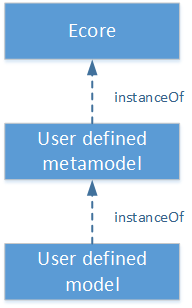
\includegraphics[width=40mm,keepaspectratio]{figures/ECore-Metamodel-Levels.png}
\caption{Different meta levels}
\label{fig:ECore-Metamodel-Rel}
\end{figure}

On the image it is clearly visible that the concepts metamodel and instance model
all depend on the perspective. From the perspective of ECore, ECore is a
metamodel while an ECore based user defined model is its instance model. From
the perspective of the user defined metamodel, it is a metamodel, while its
instance is an instance model.

The typical EMF workflow is to define a metamodel which describes the structured
data used in the application, generate the \Java{} code from it and then create
the data (instance model).

A metamodel is built using the following components (as described in ECore):

\begin{itemize}
  \item \emph{EClass} - Represents a class which can have attributes, references
  and operations. The instance model will consist of the instances of EClasses.
  \item \emph{EAttribute} - Describes an attribute which has a name and a type.
  For example an EClass can have an attribute \emph{Name} which has a type of
  \emph{String}.  
  \item \emph{EDataType} - Represents a user defined type. These are mostly used
  if none of the types described in ECore is suitable. EDataTypes allow for a
  mapping to simple \Java{} types.
  \item \emph{EReference} - Describes a relationship between two objects.
  Each reference has a name, a target EClass and a multiplicity. In addition
  there are multiple flags which can further customize the reference, from which
  the most important is the one called aggregation which decides whether this
  reference is a containment.
  \item \emph{EOperation} - These represent operations which can run on any
  instance of the containing EClass. These are sparsely used since they are
  cumbersome to work with.
  \item \emph{ESuperType} - Describes a parent-child relationship between two
  EClasses. This is the same as inheritance in object oriented programming
  languages.
\end{itemize}

The \EMF{} code generator is capable of generating the \Java{} classes from the
ECore model. Each Java class representing the EClasses defined in the ECore
model extends the EObject \EMF base class. This class provides a powerful
reflective API, with which it is possible to generically access the data of an
EClass instance without knowing its type. In addition it is also possible to
register listeners for notification on model events, like a new model element
appearing, a model element disappearing or a property getting changed.

\subsection{Metamodel example}

The purpose of this section is to show an example of a metamodel. This
metamodel will be used in the examples later in the thesis. Figure
\figref{School_Metamodel} shows a metamodel that describes the structure of
schools.

\begin{figure}[!ht]
\centering
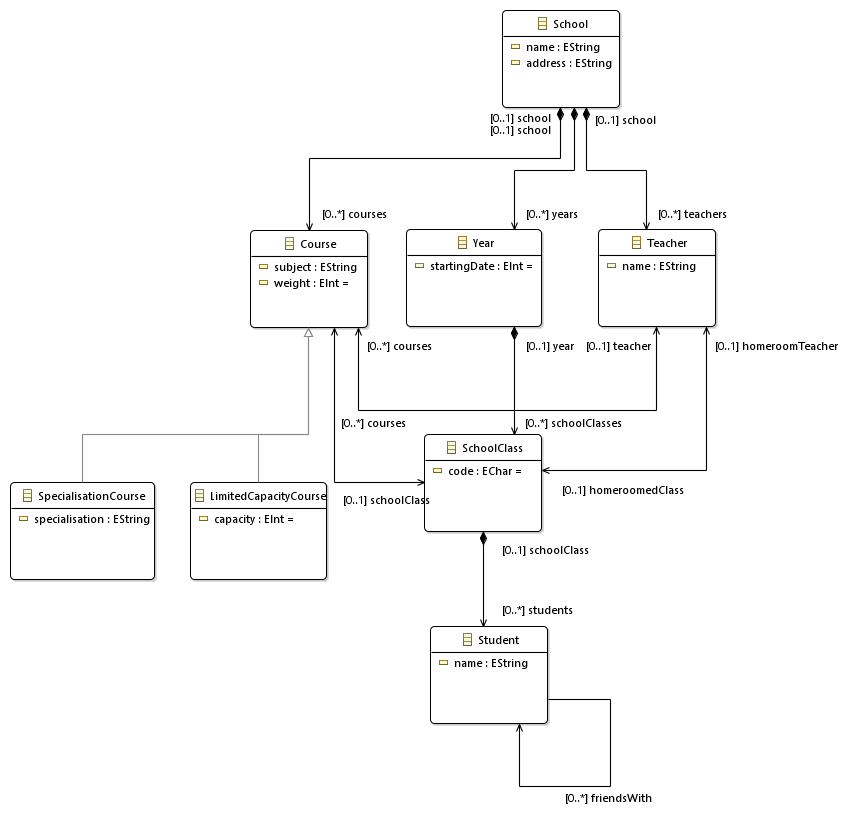
\includegraphics[width=133mm,keepaspectratio]{figures/school_class_diagram.png}
\caption{Metamodel of schools}
\label{fig:School_Metamodel}
\end{figure}

On the metamodel, some of the already explained parts of EMF can be seen. The
top element of the model, \emph{School} is an \emph{EClass}, while its
\emph{name} is an \emph{EAttribute}. School has an \emph{EReference}
\emph{teachers} to the type \emph{Teacher} with a multiplicity of ``*''. This
EReference is a containment reference, marked by the small rhombus at the start
of the arrow. There is also an example of \emph{ESuperType} between
\emph{Course} and \emph{LimitedCapacityCourse}.

The root of the model is a school which has a name and an address. Each school
can have multiple teachers, years and courses. A year represents a school year,
has a starting date and contains several school classes. Each school class
has an identifying code and a single homeroom teacher, while each teacher can
only be the homeroom teacher of one class. A school class can have multiple
courses, while a course can only be taught to a single class. Each course has a
single teacher. A course can be either regular course which has a subject and a
weight, a specialization course which has a specialization in addition or a
limited capacity course which has a capacity. A school class has several
students and each students can have multiple friends. In the case of this
metamodel, most reference has an opposite reference, meaning it can be navigated in both directions.

\begin{figure}[!ht]
\centering
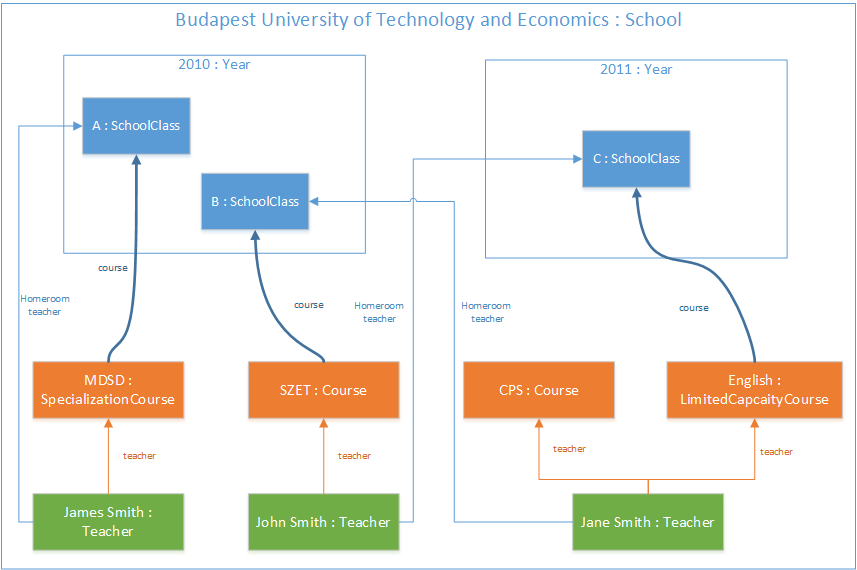
\includegraphics[width=133mm,keepaspectratio]{figures/InstanceModel.png}
\caption{A school instance model}
\label{fig:InstanceModel}
\end{figure}

Figure \figref{InstanceModel} depicts an instance model of the school metamodel.
The root of the model is a school instance with the name Budapest University of
Technology and Economics. It has two year instances, 2010 and 2011.
One year has 2 while the other has 1 school class. The school has 4 courses of
which one is a limited capacity course and another one is a specialization
course. Each course has a teacher and all of those teachers homeroom a class.

\pagebreak

Image \figref{InstanceModel_Eclipse} shows the same instance model, but as seen
inside the eclipse editor generated by EMF. The structure is clearly visible,
however the additional detail like references and attributes can not be
determined from it. There is a separate properties view that allows editing of
those information for the selected model element that is not shown on the
picture.

\begin{figure}[!ht]
\centering
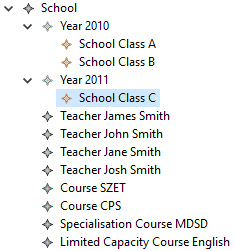
\includegraphics[width=50mm,keepaspectratio]{figures/InstanceModel_Eclipse.png}
\caption{A school instance model in eclipse}
\label{fig:InstanceModel_Eclipse}
\end{figure}

%----------------------------------------------------------------------------
\section{EMF-IncQuery}\label{sec:EMF-IncQuery}
%----------------------------------------------------------------------------

\emph{\EIQ{}}\cite{EIQ} is a framework which allows for the execution of
\emph{declarative} queries over EMF models. These queries can be defined using
\EIQ{}'s own high level yet powerful query language. The main advantage of
the declarative query language is that it is not necessary to implement complex
model traversal algorithms in an imperative programming language (like \Java{})
to perform queries.

Queries defined via \EIQ{} can be easily tested development time, thanks to its
rich tooling support. \EIQ{} generates \Java{} code for each
defined query which enables the user to run the queries over any EMF
instance model.

\subsection{The \EIQ{} Pattern Language}

The \EIQ Pattern Language is a high level, declarative graph pattern query
language. It has several advanced features of which this subsection of the
document will attempt to describe a few. All the examples will use the metamodel
shown on figure \figref{School_Metamodel}.

The following listing (\listref{SimpleIQPLExample}) shows the contents of a
simple \EIQ pattern definition file. The file begins with a package declaration
similar to \Java. The next line is an import, which imports the school metamodel
so \EIQ knows which metamodel is used.

The file has a single pattern definition named \emph{schools}. Each pattern
definition starts with the keyword \emph{pattern}, then has a name and by the
end has a parameter list. After these comes the pattern body. In this simple
case the pattern body simply declares that the parameter school has a type of
School, thus this pattern returns all school instance in a model.

\begin{lstlisting}[frame=single, language=IQPL,
label=listing:SimpleIQPLExample, caption=A simple query defined in \EIQ pattern
language]
package hu.bme.mit.cpp.localsearch.school.query

import "http://school.ecore"

pattern schools(school) {
	School(school);
}
\end{lstlisting}

The next listing (\listref{NavigationIQPLExample}) shows an example of a
navigation along a reference. In this case the results will be each
teacher-school pairs where the teacher teaches at the school.

\begin{lstlisting}[frame=single, language=IQPL,
label=listing:NavigationIQPLExample, caption=An example of a query along
reference] 
pattern teachersOfSchool(teacher, school) {
	School.teachers(school, teacher); 
}
\end{lstlisting}

Listing \listref{PatternCallIQPLExample} shows examples of calling positive and
negative pattern calls. In this example \emph{coursesOfTeacher} is called in a
positive manner from \emph{classesOfTeacher}. This basicly means copying the
body of \emph{coursesOfTeacher} in \emph{classesOfTeacher} while switching the
internal parameters to the local ones. The third pattern,
\emph{teacherWithoutClass}, uses negative pattern call, which means the called
pattern must not have a match with the provided parameters.

\begin{lstlisting}[frame=single, language=IQPL,
label=listing:PatternCallIQPLExample, caption=Pattern call example] 
pattern coursesOfTeacher(teacher, course) {
	Teacher.courses(teacher, course);
}

pattern specializationCoursesOfTeacher(teacher, course) {
	Teacher.courses(teacher, course);
	SpecializationCourse(course);
}  
 
pattern classesOfTeacher(teacher, schoolCourse) {
	find coursesOfTeacher(teacher, course);
	Course.schoolClass(course, schoolCourse);
}
 
pattern teacherWithoutSpecializationCourse(teacher) {
	neg find specializationCoursesOfTeacher(teacher, schoolCourse); 	
}
\end{lstlisting}

The following listing (\listref{AdvancedIQPLExamples}) shows examples to some of
the advanced pattern language features. The first query shows the usage of check
expressions. These allow simple Java-like expressions resulting in a boolean to
run within a query. The second pattern is an example of a disjunction where if
one of the bodies match the model that means a valid result.

\begin{lstlisting}[frame=single, language=IQPL,
label=listing:AdvancedIQPLExamples, caption=Advanced queries] 
pattern courseWithNameLongerThanWeight(course) {
	Course.subject(course, name);
	Course.weight(course, weight);
	check(name.length > weight); 
}

pattern friendlyTo(student1, student2) {
	Student.friendsWith(student1, student2);
} or {
	Student.friendsWith(student2, student1);
}
\end{lstlisting}

There are some more advanced features of the query language which I will not
detail like transitive closures and match counting, since they will not be
relevant.

\subsection{\EIQ{} API}

\EIQ{} provides an easy to use API to use the queries defined using the pattern
language. The API consists of classes provided by \EIQ{} and the generated code.
For each pattern definition, the following classes will be generated:

\begin{itemize}
  \item \emph{Match} - Represents a match for a specific query. A match contains
  references to elements from the queried model that match the current query.
  It is also possible to create a partial Match, where the user defines part of
  the references. This can be used to run \emph{bound} queries, which searches
  for matching patterns while taking into account the user defined elements.
  \item \emph{Matcher} - One of the most important classes, it starts the
  pattern matching of a specific query definition. The results of a pattern
  match can also be accessed through this class, while it also provides
  different views over the results.
  \item \emph{Processor} - This is an abstract helper class with a
  \emph{process} method. A user implemented MatchProcessor can be passed to a
  Matcher, which will call the process method using each match as a parameter.
  \item \emph{Evaluator} - These classes are helper classes to evaluate checks,
  they should not be used by the user.
  \item \emph{QuerySpecification} - The specification of a query which can also
  instantiate a matcher.
\end{itemize}

Listing \listref{EIQApiUsage} shows example of using the \EIQ{} API. The first
step is to create an \emph{EMFScope} from the EMF instance model. This is a
simple wrapper over anything that can be considered an EMF model. The next step
is to initialize an \emph{IncQueryEngine} over the newly created scope. After
this a \emph{Matcher} can be asked from the engine using the patterns
\emph{QuerySpecification}. The matcher allows the usage of a \emph{Processor} to
process each match. In this case, every schools name will get printed out on the
console.

\begin{lstlisting}[frame=single, language=Java,
label=listing:EIQApiUsage, caption=Usage of the \EIQ{} API] 
IncQueryEngine engine = IncQueryEngine.on(new EMFScope(model));

SchoolMatcher matcher = engine.getMatcher(SchoolQuerySpecification.instance);

matcher.forEachMatch(new SchoolsProcessor() {
	@Override
	public void process(final School school) {
		System.out.println(school.getName());
	}
});
\end{lstlisting}

%----------------------------------------------------------------------------
\section{Xtend}\label{sec:Xtend}
%----------------------------------------------------------------------------

Xtend\cite{Xtend} is a statically typed dialect of \Java{} which compiles into
human readable \Java{} code. The language has its roots in \Java{} but improves on
many aspects of it:

\begin{itemize}
  \item \emph{Extension methods} - allows adding new methods to closed types
  without modifying them
  \item \emph{Lambda expression} - Lambda expression is a code snippet wrapped
  in an object that can be passed around easily. This was a more important
  feature before \Java 8 since it allowed a more concise way of passing around
  methods (instead of anonymous classes), but it still improves over \Java 8
  lambdas since they can be used in place of abstract classes, not only
  functional interfaces.
  \item \emph{Active annotations} - Using active annotations, the \Java code
  compilation can be customized.
  \item \emph{Template expression} - These allow easy parametrization of
  strings. This feature is most useful for generating code.
  \item \emph{Type inference} - Xtend can usually infer the types of variables,
  methods thus reducing code size (especially in case of generics).
  \item \emph{Properties} - Xtend interprets setters and getters as properties,
  which makes accessing and writing properties of classes less cumbersome since
  they can be accessed by their name (i.e., instead of calling
  obj.getName() one can access name using obj.name).
  \item \emph{Operator overloading} - In Xtend it is possible to overload
  operators for any type. It is mostly useful for mathematical computations with
  BigInteger or when writing math library using vectors and matrices.
\end{itemize}

Since Xtend compiles to \Java code there is no interoperability issue between
\Java libraries and Xtend code or vice versa.

\subsection{Xtend example}

For introduction, listing \listref{XtendIntro} shows the previous \EIQ API usage
example code (\listref{EIQApiUsage}) translated to XTend. There are several
small differences like static access is done through ``::``, no ``;'' at end of
line or using ``val'' instead of type, but the most significant difference is
the usage of lambda expression in \emph{forEachMatch}. In this case, the lambda
expressions parameter is a \emph{SchoolMatch} that has a school property. In
lambda expressions if they only have a single parameter, then the parameter's
scope is accessible in the local scope, so basically it is possible to access
school without writing out the parameters name and the dot. It is also notable
that properties can be accessed directly, there is no need to write getName().

\begin{lstlisting}[frame=single, language=Xtend,
label=listing:XtendIntro, caption=Usage of the \EIQ{} API with Xtend] 
val engine = IncQueryEngine::on(new EMFScope(model))

val matcher = engine.getMatcher(SchoolQuerySpecification::instance)

matcher.forEachMatch[println(school.name)]
\end{lstlisting}

Xtends most important feature in my case was its code generation capability
through template expressions, to which listing \listref{XtendCodeGen} gives an
example. This example generates a simple \CPP{} program which prints out a
greeting. The most important things are how the string between the triple ticks
maintains its indentation and how easy it is to parametrize the text.

\begin{lstlisting}[frame=single, language=Xtend,
label=listing:XtendCodeGen, caption=Xtend code generation] 
def genCppGreeting(String... names) ```
	#include <iostream>

	int main(int, char**) {
		�FOR name : names�
		std::cout << "Hello �name�!" << std::endl;
		�ENDFOR�
	}
```
\end{lstlisting}
\chapter{Local Search}


With the spread of \emph{Model Driven Engineering} paradigms, more and more
tools appear to facilitate it. A common problem these tools face is the
efficient querying of graph patterns on the models. There are two main approach
to this problem with different benefits and drawbacks:

\begin{itemize}
  \item \emph{Local Search} - in this approach, the pattern matching is driven
  by a search plan, which contains simple checks and binding operations.
  \item \emph{Incremental Graph Matching} - this approach maintains a cache
  for the patterns based on the model while listening to any changes to the
  model and updating the caches as required.
\end{itemize}

For the problem of running graph matching algorithms in \emph{C++} over object
instances in an efficient manner, the local search based approach is easier to
implement, since it does not require notifications for object instance
lifecycle.

%----------------------------------------------------------------------------
\section{Pattern body graph}\label{sec:PatternBodyGraph}
%----------------------------------------------------------------------------

A \emph{pattern body graph} is a graphical representation of a graph pattern.
Figure \figref{patternBodyGraph} shows the pattern body graph of the previously
introduced pattern \emph{specializationCoursesOfTeacher}
(\listref{PatternCallIQPLExample}). On the pattern body graph, there are three
pattern variables, \emph{teacher}, \emph{course} and \emph{C}. The variable
teacher is constrained to be of Teacher type, while course is of Course type.
Variable C is an edge, and it's type is the courses association between Teachers
and Courses. The course variable is further constrained to be a
SpecializationCourse.

\begin{figure}[!ht]
\centering
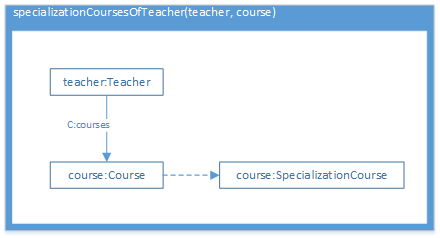
\includegraphics[width=110mm,
keepaspectratio]{figures/pattern_body_graph.png}
\caption{Pattern body graph of \emph{specializationCoursesOfTeacher}}
\label{fig:patternBodyGraph}
\end{figure}

%----------------------------------------------------------------------------
\section{Search graph}\label{sec:SearchGraph}
%----------------------------------------------------------------------------

The search graph is a graph based data structure of constraints and variables
for representing a query over a model. The search graph is a hypergraph, it's
edges represent constraints and nodes represent pattern variables. From the
original pattern graph, each node and edge turns into a pattern variable. The
constraints connect the constraints and arguments of the pattern graph, for
example if a constraint has a source and a target argument, the 3 nodes will be
connected with a source and a target edge.

This graph representation is very useful, since it allows for easy
simplification and normalization steps, which enhance the efficiency of the
query.

\begin{figure}[!ht]
\centering
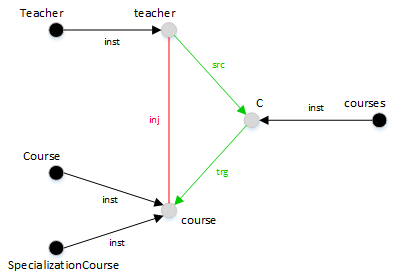
\includegraphics[width=110mm,
keepaspectratio]{figures/search_graph.png}
\caption{Search graph of \emph{specializationCoursesOfTeacher}}
\label{fig:searchGraph}
\end{figure}

Figure \figref{searchGraph} shows an example of the search graph of the
\emph{specializationCoursesOfTeacher} pattern. The search graph has seven
pattern variables. Pattern variables \emph{teacher}, \emph{course} and \emph{C}
represent variables (denoted by grey dots), while \emph{Teacher},
\emph{Course}, \emph{SpecializationCourse} and \emph{courses} represent types
(denoted by black dots). Between pattern variables and types, there are
\emph{``instance of''} constraints (black edges marked by \emph{inst}). Green
edges define the source and target of an edge (on the original pattern body
graph). Each node and each edge pattern variable from the pattern body graph
gets connected with an \emph{injectivity} constraint (red edge marked by \emph{inj}), meaning they
cannot be assigned the same value even if the other constraints would allow it.
Since there is only one edge pattern variable on the graph, there is no
injectivity constraint for it.

%----------------------------------------------------------------------------
\section{Search plan}\label{sec:SearchPlan}
%----------------------------------------------------------------------------

During the matching process, the search graph gets transformed into a search
plan. The transformation steps are shown on figure \figref{graph_to_plan}.

\begin{figure}[!ht]
\centering
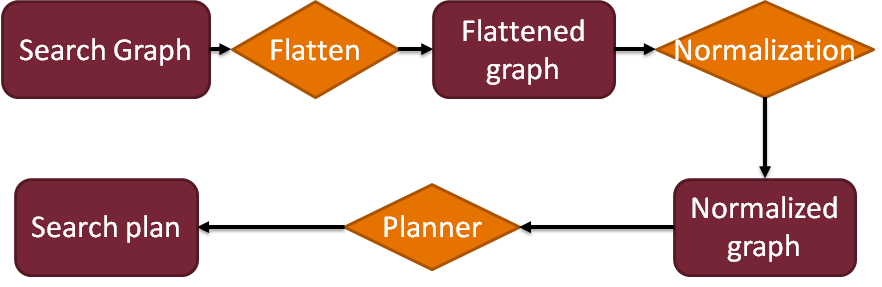
\includegraphics[width=130mm,
keepaspectratio]{figures/search_graph_plan_trans.png}
\caption{Search graph to search plan transformation}
\label{fig:graph_to_plan}
\end{figure}

The search graph may contain references to other queries. These references are
removed in the flattening step, where each reference is replaced with the
specified queries search graph. This results in the flattened search graph. The
next step is the normalization step. This removes any constraint deducable from
the metamodel, removes any duplicate or trivial constraints. The normalized
graph then gets sent to the planner which produces the search plan. 

The search plan is an ordered list of operations consisting of simple actions
applied to the model. The search graph have two basic types of operation:

\begin{itemize}
  \item extend - these operations assign a value to a variable based on a
  constraint. For example if a variable has a type constraint, then an object of
  the specified type will be bound to it.
  \item check - these kind of operations check whether the specified
  constraints are met on already bound variables, e.g. in case of a type
  constraint it checs if whether the object assigned to the variable is the
  specified type.
\end{itemize}

Executing the operations of the search plan in order while backtracking if an
operation fails results in objects assigned to the pattern variables which
satisfy the constraints.

\chapter{Architecture and Design}

This chapter's aim is to familiarize the user with the design decisions and the
architecture of the application, describe the challeenges encountered during
development and provide solutions to some of them.

%----------------------------------------------------------------------------
\section{Architecture}\label{sec:Architecture}
%----------------------------------------------------------------------------

The application's components can be separated into three main categories:

\begin{itemize}
  \item Java-Compile Time - components that are used while designing the
  queries and generating code.
  \item \CPP{} Compile Time - the generated code.
  \item \CPP{} Runtime - the code running the queries.
\end{itemize}

The architecture of the application is shown on figure \figref{architecture}.
The main component of the architecture is the ECore model, which serves as
the description of the possible object types and their relationships.
In my case this is basically similar to an UML class diagram. Further
detail will be discussed in chapter \sectref{CppObjectModel}.

\begin{figure}[!ht]
\centering
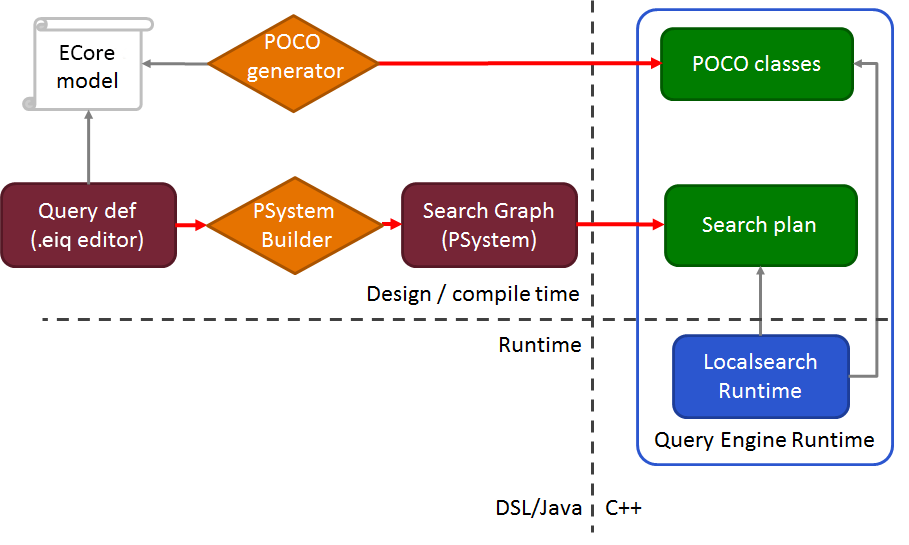
\includegraphics[width=150mm, keepaspectratio]{figures/architecture.png}
\caption{The architecture of the engine}
\label{fig:architecture}
\end{figure}

From the ECore model, the POCO generator (\sectref{GeneratedCodeStructure})
generates the \CPP{} classes. These are the classes the runtime model consists
of and the queries can be executed on.

Writing queries is supported through the \EIQ{} pattern language editor, which
provides content assist, syntax highlighting, validation and several other
features to help the user in query development.

From the query definition the search graph (called \emph{PSystem} in
\EIQ{}) gets transformed. This search graph contains every information
necessary to create the search plan. The search plan gets transformed from the
search graph to Java first, then based on this plan the actual search operations
get transformed into \CPP{} code. The available search operations and their
execution is coded in a runtime library. The assembly of the actual search plan
and its execution gets obfuscated by generated code, the user only has to call
the appropriate generated method to get the matching elements to a specific query.

This architecture makes it so that the user has no interaction with any
localsearch related part of the application, i.e. he has to create the model,
write the queries and later on call the queries in his \CPP{} application,
everything else is handled hidden from him.

\section{EMF to \CPP{} generation} \label{sect:CppObjectModel}

This section focuses on the ECore metamodel used to describe the class hierarchy
of the generated code and the structure of the generated code.

%----------------------------------------------------------------------------
\subsection{Metamodel}\label{sec:Metamodel}
%----------------------------------------------------------------------------

\begin{figure}[!ht]
\centering
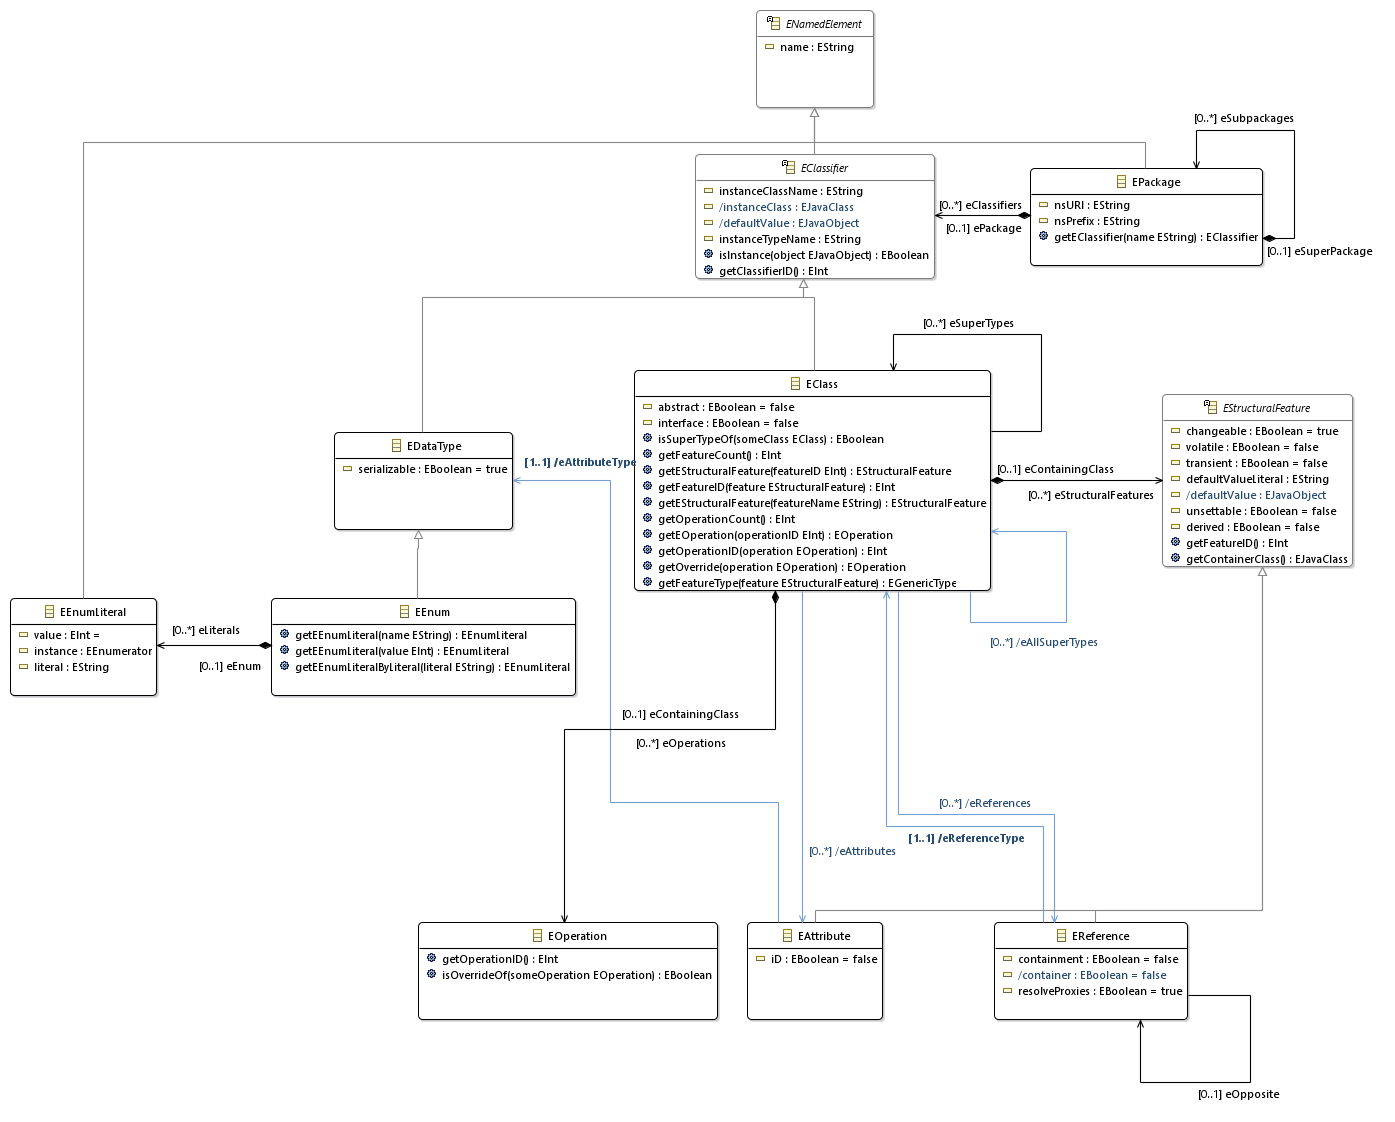
\includegraphics[width=160mm, keepaspectratio]{figures/ecore_diagram.png}
\caption{The ECore Class diagram metamodel}
\label{fig:metamodel}
\end{figure}

The metamodel (as seen on figure \figref{metamodel}) is a simplified version of
the ECore metamodel. Ecore is a reference implementation of OMG's MOF
standard. It allows expressing other models while it is its own metamodel,
meaning ECore is defined using its own concepts. The root of ECore is
\emph{EPackage}, which is a simple container for organization purposes. It
may contain other EPackages or \emph{EClassifiers}, which can either
be an \emph{EClass} or an \emph{EDataType}. An EDataType are primitive types
like integer, string or enum, which corresponds to \emph{EEnum}. An EEnum may
contain multiple literals represented by \emph{EEnumLiteral}. An EClass serve as
a class in object oriented programming (OOP). It can be a regular class, an
abstract class or an interface, corresponding to the respective meaning in OOP.
An EClass contains EStructuralFeatures. An EStructuralFeature may either be an
\emph{EReference}, an \emph{EAttribute} or an \emph{EOperation}. An EReference
is an association between two EClasses, which may be a containment reference
meaning the source of the reference contains the value of the actual object or
objects referenced. Each EReference may possess an \emph{eOpposite} if there is
an EReference in the opposite direction. An EAttribute represents a simple
primitive type attribute for a EClass, like an integer, string, boolean etc. An
EOperation corresponds to a function declaration. Defining a function is not
directly supported by the metamodel.

%----------------------------------------------------------------------------
\subsection{Generated code structure}\label{sect:GeneratedCodeStructure}
%----------------------------------------------------------------------------

To talk about the generated code structure, it is necessary to have an actual
model to generate the code from. For this purpose, I used the previously
introduced school model shown on figure \figref{School_Metamodel}. The structure
of the generated code can be seen on figure \figref{GenCodeStruct}.

\begin{figure}[!ht]
\centering
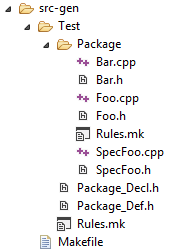
\includegraphics[width=40mm, keepaspectratio]{figures/gen_code_struct.png}
\caption{The generated code structure}
\label{fig:GenCodeStruct}
\end{figure}

The model school got generated into a folder named accordingly inside the
cpp-gen folder of the project. For every EPackage  a folder and two header files
are created. The header file postfixed with \emph{def} contains includes to
the definition of the classes inside the package, while the one postfixed with
\emph{decl} contains the declaration of said classes. The folder created for the
package contains header and source files for each EClass and, if there are any,
the above explained files for contained EPackages. To help with compilation, a
makefile also gets generated. The root model folder has the makefile itself,
which then includes the rule files in the folders recursively. This way the
users only job is to create the main file and the code can be easily compiled.
Another way to use the generated code would be to simply include the rule file
in the user's own makefile in another project. This gives great flexibility to
anyone using a make based build tool.

\section{Runtime Library}

This section will mostly focus on the implementation specific details of the
\CPP{} local search runtime, such as problems specific to \CPP{} and their
solutions, the structure of a search plan, its operations and their execution.

%----------------------------------------------------------------------------
\subsection{\CPP{} specific problems}\label{sect:CppSpecificProblems}
%----------------------------------------------------------------------------

In the case of the runtime, \CPP{} brought with its speed several problems, such
as the lack of any reflection API and a unified object base class. This caused
several issues during the implementation, because running local search over \CPP{}
objects requires instance checking, getting fields by name to navigate
associations and iterating over every instance of a specific task. This section
will propose a solution for each of the above mentioned issues.

%----------------------------------------------------------------------------
\subsubsection{Objects in \CPP{}}\label{sect:ObjectsInCpp}
%----------------------------------------------------------------------------

During the local search process it is necessary to hold every single object in
containers without knowing their type. In \CPP{} there are three main ways to do
this.

\begin{itemize}
  \item using heterogeneous collections with a common base class
  \item \emph{void*} pointer
  \item wrapper object
  \item using templates
\end{itemize}

Using a common base class is probably the easiest and most obvious solution,
but it would constraints the type of objects the local search runtime can
be used on which makes this solution undesirable.

Using \emph{void*} pointers would mean the complete loss of type information,
thus making any dynamic type checking mostly impossible. This alone makes this
solution unusable.

The third method of using wrapper object is a possible solution with the
only drawbacks of being complicated, slow and memory inefficient.

The last, template based version is probably the most complicated one. It
requires complicated template programming which results in slower compile times
and larger executables, but it has a superior runtime speed and memory usage to
all other alternatives.

\textbf{Wrapper object based solution}

 The structure of the wrapper object can be seen on figure
 \ref{fig:wrapper_structure}.

\begin{figure}[!ht]
\centering
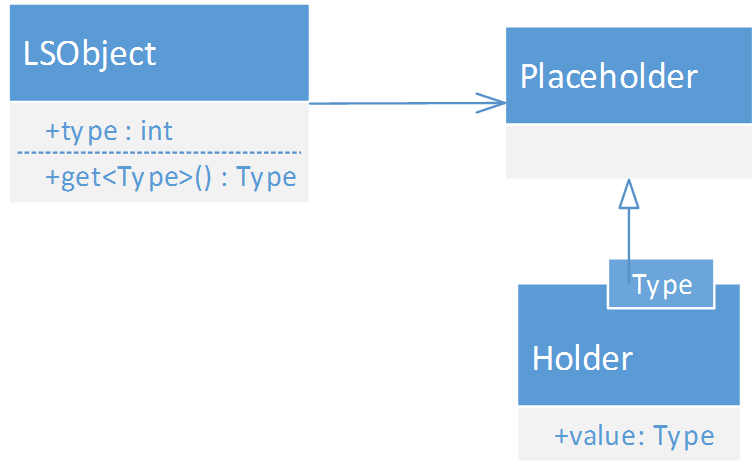
\includegraphics[width=70mm, keepaspectratio]{figures/wrapper_structure.png}
\caption{The structure of the wrapper object}
\label{fig:wrapper_structure}
\end{figure}

The \emph{LSObject} (Local Search Object) contains the type information, a
template method to get the value contained cast to the proper type and a pointer to a
\emph{Placeholder} object. The actual object contained is actually of the
\emph{Holder} template type, which contains the original value. The placeholder
object's construction can be seen as below.

\begin{lstlisting}[frame=single,float=!ht,language=C++, caption=Constructing a
wrapper object] template<typename T>
LSObject(const T& value, int type) :
	_ptr(new Holder<T>(value)), type(type) {
}
\end{lstlisting}

As it can be seen from the code, the \emph{LSObject}'s holder will hold a
reference to the value, be it pointer or actual value. The second parameter
\emph{type} contains the type information for the value. 

\begin{lstlisting}[frame=single,float=!ht,language=C++, caption=Retrieving
correctly typed object]
template<typename T>
inline T& LSObject::get() const {
    return static_cast<Holder<T>&>(*this->_ptr).value;
}
\end{lstlisting}


The \emph{get} method of the wrapper object returns the value as it was passed
in, however this require the compile time knowledge of the original type. The
implementation can be seen below:

The usage of the wrapper class is shown in listing \listref{wrapper_usage}.

\begin{lstlisting}[frame=single,float=!ht,language=C++,
label=listing:wrapper_usage, caption=Wrapper object usage]
Foo f;
f.Name = "Foo1";
LSObject ls_f(f, 0);

ls_f.get<Foo>().Name
\end{lstlisting}

The design of the class was heavily inspired by the
\emph{boost::any}\cite{boost-any} class.

The main problem with this approach is its speed. The speed issue is caused by
the fact that while iterating over the instances of a class, they all have to be
wrapped in a wrapper class while creating a new collection. This costs a
considerable amount of time. Also for this reason, the memory footprint of this
solution is considerably higher.

\textbf{Template based solution}

This solution needed the most effort in implementation, since this requires
the type information to flow through the whole runtime. The main idea of the
solution is that all components of the engine have several template parameters
to describe the types it has to handle. The listing \listref{template_example}
contains the declaration of a navigation class, which shows how complicated
class declarations can get using this approach.

\begin{lstlisting}[frame=single,float=!ht,language=C++,
label=listing:template_example, caption=Template based approach example]
template<typename SrcType, typename TrgType, typename Collection, 
		typename Member, typename MatchingFrame>
class NavigateMultiAssociation
  : public ExtendOperation<TrgType, Collection, MatchingFrame>;
\end{lstlisting}

The main benefits of this solution are speed and really low memory usage. The
speed is gained from the fact that, with this approach, iterators can be used
over the original instances collections without any wrapping, and only
filtering is necessary. This also means that the memory usage scales with
pattern complexity and is completely independent of model size.

%----------------------------------------------------------------------------
\subsubsection{Iterating class instances}\label{sect:IteratingClassInstances}
%----------------------------------------------------------------------------

To allow iteration over all instances of a class, a registry needs to be managed
which gets updated on each instance construction or deletion. The only feasible
way to do this is to write the classes constructor and destructor in a way that
it adds new instances to a list when they are created and removes them when they
are deleted. This method limits the type of objects the runtime works on, but
this is the most reasonable solution. An example of a class prepared to count
its instances can be seen below.

\begin{lstlisting}[frame=single,float=!ht,language=C++]
class Foo  {
public:
	Foo() {
		_instances.push_back(this);
	}
	
	~Foo() {
		_instances.remove(this);
	}
		
	static std::list<Foo*> _instances;
};
\end{lstlisting}

This solution uses the \emph{std::vector} to contain the created instances.
While the constructor is trivial the destructor is more interesting. The
check whether the destructed object is in the vector seems unnecessary, but \CPP{}
allows the allocation of memory for an object without actually calling its
constructor. This memory portion can be freed with delete which also calls the
destructor. In this case, the instance will not be in the vector and this could
cause issues.

%----------------------------------------------------------------------------
\subsubsection{Instance checking}\label{sect:InstanceChecking}
%----------------------------------------------------------------------------

In the case of \CPP{} the generally accepted way of dynamic type checking is using
\emph{dynamic\textunderscore cast} provided by the language. This is however a
not ideal solution. The first problem is it only works on dynamic classes, i.e.\
classes with at least one virtual method. The other issue is speed, as
\emph{dynamic\textunderscore cast} uses vtables to check if the specified
instance can be casted to the specified type. To illustrate the speed issues,
the following table (\ref{tab:InstPerf}) shows the results of performance tests
made in \CPP{} and Java.

\begin{table}[ht]
	\footnotesize
	\centering
	\caption{Instance of check performance comparison of Java and \CPP{}}\label{tab:InstPerf}
	\begin{tabular}{ | l | c | c |}
	\hline
	Iterations 	& Java 		& \CPP{} 		 \\ \hline
	$10^4$ 		&  1	ms 	& 0.1	ms \\
	$10^5$ 		&  11 	ms  & 1		ms \\
	$10^6$ 		&  15 	ms  & 17	ms \\
	$10^7$ 		&  41 	ms  & 173	ms \\
	$10^8$ 		&  261 	ms  & 1746	ms \\
	$10^9$ 		&  2515 ms  & 17456	ms \\
	\hline
	\end{tabular}
	\label{tab:TabularExample}
\end{table}

As the table shows, Java is slower on small number of iterations, but on higher
number of iterations the JIT compiler manages to optimize the instance checking
process and gets roughly a magnitude faster than \CPP{}.

The solution I propose is an inheritance matrix in which it is contained whether
an instance of a type is a child of another type. This can be generated using
the model of the classes. This also means that most of the calculation is done
generation time, thus making this method faster than most dynamic type
inference method provided by languages. For the following examples I will use
the class structure shown on figure \ref{fig:simple_class} . In this example
there are three classes, \emph{Foo}, \emph{Bar} and \emph{SpecFoo}.
\emph{SpecFoo} extends \emph{Foo}. The example does not contain any of
the possible more complex hierarchy structures, like diamond, but nonetheless it
supports them.

\begin{figure}[!ht]
\centering
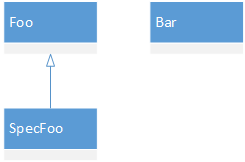
\includegraphics[width=50mm, keepaspectratio]{figures/simple_class.png}
\caption{Example class structure}
\label{fig:simple_class}
\end{figure}

To use this method, the runtime knowledge of a classes exact instance is
required. This could be done via a virtual method (which is undesirable
because of larger memory footprint for instances) or template metaprogramming.
Template metaprogramming would only work on the static type of the object, not
the dynamic, i.e. it would not work correctly with inheritance. For example for
the pointer \emph{Foo* f = new SpecFoo()} it would always return Foo as the
type, same with the built in \emph{\texttt{type\_id}} function. Thus the only
viable solution in my case is the virtual method. An implementation example for
such solution can be seen in the following example (expanding upon the
previous code sample):

\begin{lstlisting}[frame=single,language=C++, label=listing:type_id,
caption=Type identifier for classes]
class Foo  {
public:
	Foo() {
		_instances.push_back(this);
	}
	
	~Foo() {
		_instances.remove(this);
	}
	
	virtual unsigned short get_type_id() const {
        return type_id;
    }
		
	static std::list<Foo*> _instances;
	static const unsigned short type_id = 1;
};
\end{lstlisting}

In this example, the \emph{\texttt{type\_id}} is generated. This might cause
issues if the code is generated in multiple sessions. This can be solved with a
class that has a growing id for each of its instance, and a bit of template
metaprogramming. A simplified solution can be seen in listing
\listref{unique_number}.

\begin{lstlisting}[frame=single,float=!ht,language=C++,
label=listing:unique_number, caption=Unique number generation for type
identifiers]
class unique_number { 
public:
	unique_number(): cur_id(max_id++) {}

private:
	static unsigned long max_id;
	unsigned long cur_id;
};

template<typename C>
struct type_number {
	static unique_number number;
};

class Foo  {
	...
	virtual unsigned short get_type_id() const {
        return type_number<Foo>::number;
    }
	...
};
\end{lstlisting}

The basic idea is that every instance of \emph{\texttt{unique\_number}} contains
a unique identifier. For each class, a separate \emph{\texttt{type\_number}}
gets created compile time with a \emph{\texttt{unique\_number}} inside, which can be
retrieved in the \emph{\texttt{get\_type\_id}} method. This guarantees a unique
id for each class that's calculated compile time.

Using this type id as an identifier it is possible to create a boolean matrix
(two dimensional array) of the type relationships. For each member of this matrix
'm' 
\[
m[type1][type2] = type1\textrm{ instanceof }type2
\]

In the case of the presented example this matrix would look like in the
following table (\ref{tab:InhMatrix}):

\begin{table}[ht]
	\footnotesize
	\centering
	\caption{Example inheritance matrix}\label{tab:InhMatrix}
	\begin{tabular}{| c | c | c | c |}
	\hline
			& Foo	& Bar	& SpecFoo	\\ \hline
	Foo		& true	& false	& false		\\ \hline
	Bar		& false	& true	& false		\\ \hline
	SpecFoo	& true	& false	& true		\\ \hline
	
	\hline
	\end{tabular}
	\label{tab:TabularExample}
\end{table}

The diagonal of the matrix is obviously true (since an instance of Foo is
trivially the instance of Foo). The SpecFoo instance is the instance of both Foo
and SpecFoo.

This method allows instance checking to be done in basically two array indexing
operations. From my performance measurements, this method seem to be marginally
faster than the Java \emph{instanceof} operation.

\begin{table}[ht]
	\footnotesize
	\centering
	\caption{Instance of check performance comparison of Java,
	\CPP{} and inheritance matrix}\label{tab:InstPerf}
	\begin{tabular}{ | l | c | c | c |}
	\hline
	Iterations 	& Java 		& \CPP{}	&	Inheritance Matrix	\\ \hline
	$10^4$ 		&  1	ms 	& 0.1	ms	&	0.03	ms			\\
	$10^5$ 		&  11 	ms  & 1		ms	&	0.3		ms			\\
	$10^6$ 		&  15 	ms  & 17	ms	&	3		ms			\\
	$10^7$ 		&  41 	ms  & 173	ms	&	15		ms			\\
	$10^8$ 		&  261 	ms  & 1746	ms	&	172		ms			\\
	$10^9$ 		&  2515 ms  & 17456	ms	&	1725	ms			\\
	\hline
	\end{tabular}
	\label{tab:TabularExample}
\end{table}

%----------------------------------------------------------------------------
\subsubsection{Navigation through associations}
\label{sect:NavigationThroughAssociations}
%----------------------------------------------------------------------------

Navigation through associations specified by their name requires meta
information about the classes. This information can be accessed using the \CPP{}
feature called \emph{pointer to member}. A pointer to member is similar to a
function pointer in that they allow the calling of a member function without
knowing its name. Yet, unlike ordinary an ordinary pointer to function, it also
enables the manipulation of data members of an object.

The following listing (\listref{p2m_decl}) shows an example of a pointer to
member declaration. In this case, a pointer to a member of the \emph{Teacher}
class is declared, which member has a \emph{std::string} type.

\begin{lstlisting}[frame=single,float=!ht,language=C++,
label=listing:p2m_decl, caption=Pointer to member declaration]
std::string Teacher::*name;
\end{lstlisting}

A pointer to member can be initialized to any member of the declared class with
the declared type. Listing \listref{p2m_init} shows how to do so.

\begin{lstlisting}[frame=single,float=!ht,language=C++,
label=listing:p2m_init, caption=Pointer to member initialization]
std::string Teacher::*name = &Teacher::name;
\end{lstlisting}

This pointer to member can be passed around to functions as parameter. With
this, it is easy to implement a simple method which navigates over an
association for any class. An example of such a method is shown in listing
\listref{p2m_usage}.

\begin{lstlisting}[frame=single,float=!ht,language=C++,
label=listing:p2m_usage, caption=An universal navigation method using pointer
to member] 
template<SrcType, TrgType, Member>
TrgType navigate(SrcType src, TrgType Member::* navigator) {
  return src->*navigator;
}
\end{lstlisting}

In this example, it is assumed that \emph{Member} and \emph{SrcType} is the
same. In a more realistic use case, the variable \emph{src} has to be casted to
either \emph{Member} or \emph{Member*} depending on weather \emph{SrcType} was a
pointer or value (which can be determined through template metaprogramming).

%----------------------------------------------------------------------------
\subsubsection{Missing value representation}
\label{sect:MissingValueRepresentation}
%----------------------------------------------------------------------------

The query APIi uses Match class instances to represent the query results. These
classes are basically tuples which contain all the data related to a query
result. As the API supports querying of a single arbitrary match, it is
necessary to represent a missing value. This could be done using nullptr, but
that would require the result object to be a pointer, which means it has to be
dynamically allocated on the memory. This should be avoided, so another solution
was necessary.

The most common approach of representing a missing value is the null object
pattern. For this purpose, the runtime library contains an \emph{Optional}
class, which represents either a value or the absence of a value.

Listing \listref{optional} shows the interface of the optional class. An
optional instance can be requested through static methods, for either a missing
value or a present value. The \emph{get} method allows the retrieval of the
value or throws an error if the value is missing. It is possible to check for
the presence of a value through the \emph{present} method. There are additional
utility methods to handle the presence or absence of a value in a functional
style.

\begin{lstlisting}[frame=single,float=!ht,language=C++,label=listing:optional,
caption=Optional interface] 
template<typename T>
class Optional {
public:
        static Optional<T> empty();
        static Optional<T> of(T object);

        bool present();
        void if_present(void (*fun)(T));
        T or_else(T (*fun)());
        T or_else(T other);
        T get();
};
\end{lstlisting}

%----------------------------------------------------------------------------
\subsection{Library Architecture}\label{sect:Runtime_library}
%----------------------------------------------------------------------------

The runtime library contains several classes to facilitate the running of
queries over \CPP{} object hierarchies. A simplified version of the library
class diagram can be seen on figure \figref{runtime}.

\begin{figure}[!ht]
\centering
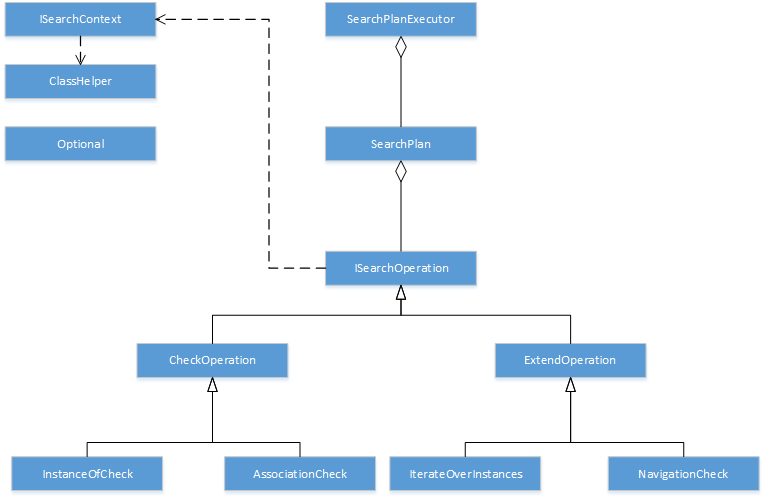
\includegraphics[width=150mm, keepaspectratio]{figures/runtime_diagram.png}
\caption{The runtime library}
\label{fig:runtime}
\end{figure}

The runtime library consists of three utility classes. The \emph{ISearchContext}
is the context of a search operation. It gives access to other utility class
instances parametrized correctly for the current search operations context. Such
utility class is the \emph{ClassHelper} which contains the dynamic instance
checking functionality described in section \sectref{InstanceChecking}. Another
utility class is \emph{Optional}, its purpose is detailed in
\sectref{MissingValueRepresentation}.

The rest of the library deals with the execution of a search plan. The central
piece of these classes is \emph{SearchPlan}. It contains an ordered list of
\emph{ISearchOperations}. An ISearchOperation can either be:

\begin{itemize}
  \item \emph{Check operation} - these type of operations receive one or more
  value and determines if a constraint is satisfied by them.
  \item \emph{Extend operation} - these operations receive zero or more values
  and based on those values calculates an additional value.
\end{itemize}

A check operation can either be an \emph{InstanceOfCheck} or an
\emph{AssociationCheck}. The InstanceOfCheck tests whether the provided value is
of the expected type. This is done as explained previously
(\sectref{InstanceChecking}). The AssociationCheck tests whether two values are
related through an association. This has two cases, if the association is [0..1]
multiplicity, this is a simple equality check, while if the association is
[0..*] then this is a list containment check.

Similarly to a check operation, the extend operation has two main types:
\emph{IterateOverInstances} and \emph{NavigateAssociation}. IterateOverInstances
simply assigns all instances of a class to a variable one by one.
NavigateAssociation gets a value and an association as a parameter and assigns
the instance or instances reached by navigating the association from the given
value to a variable.

The search plan is executed with the help of the \emph{SearchPlanExecutor}. The
search plan executor simply executes the search operations of a search plan and
returns if a match is found. This also provides an iterator with which a search
plan can be executed in a lazy manner.

\section{Generated code and API}\label{sect:generated_code_and_api}

The patterns defined with the \EIQ{} Pattern Language can be executed through
the usage of the generated classes. This chapter section goes into detail
explaining the generated classes.

The program supports two different approaches for executing the queries in the
generated code: \emph{runtime} based and \emph{iterator} based. The runtime
based fully utilizes the previously showcased local search runtime, assembles a
search plan and executes it. Meanwhile, the iterator based approach only uses a
few parts of the runtime and mostly uses built in language constructs.

\subsection{Runtime based}

This approach uses all the available runtime classes to generate a mostly easy
to understand human readable generated code where the search operations are
clearly visible. 

The generated artifacts for the runtime based approach can be seen on figure
\figref{runtime_gen}. The runtime based approach generates one header file per
query definition file and two header files for each pattern definition. 

\begin{figure}[!ht]
\centering
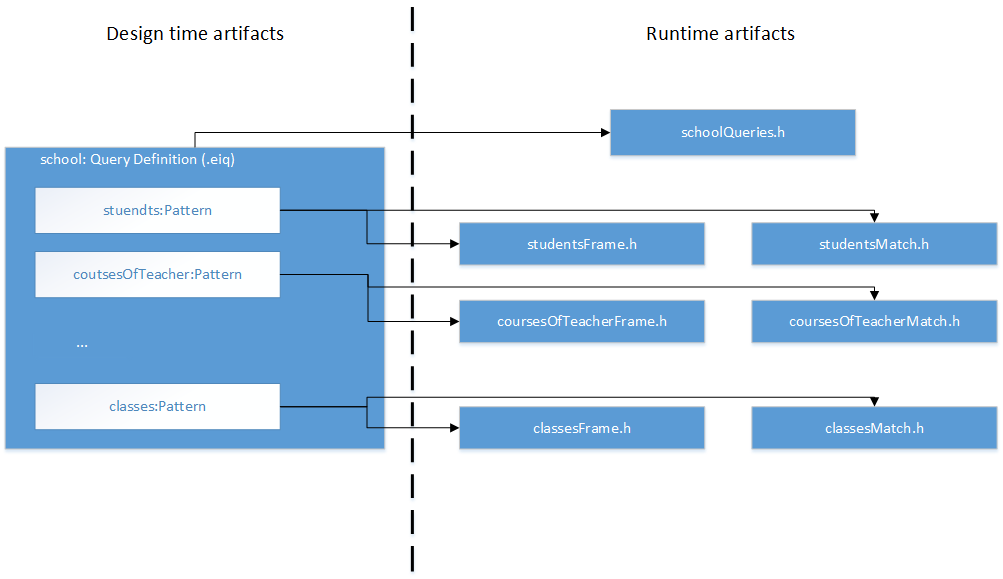
\includegraphics[width=130mm, keepaspectratio]{figures/runtime_gen_art.png}
\caption{The generated artifacts for the runtime based approach}
\label{fig:runtime_gen}
\end{figure}

The single central header file generated for a query definition file is named
after the original with the following pattern: \emph{<original .eiq name>Queries.h}.
Its function is to provide an API to call the defined patterns in multiple
ways:

\begin{itemize}
  \item \emph{get\_all\_<pattern>} - retrieves all matches for the defined pattern.
  \item \emph{get\_one\_<pattern>} - returns a single, arbitrary match for
  the defined pattern.
\end{itemize}

These methods also get generated with different parameter lists based on the
defined pattern bindings. More information about pattern bindings will be
explained in section \sectref{binding_variables}. In addition, it also contains
the initialization of the inheritance matrix which is generated from the
metamodel.

The two headers generated for a single pattern are representing a related
\emph{Frame} and a \emph{Match}. The frame is only used internally, it is a
simple struct containing all the variables used during the process of
executing the local search algorithm. The match represents a single match of the
pattern, it contains all the variables defined by the user as external variable
(defined in the patterns parameter list and not in the body), an equality
operator for the match and a hash function. The latter two are necessary to
check whether the match is unique. An additional difference between the two is
the type of the common external variables. A match always uses the strictest
determinable type from the type hierarchy, while a frame uses the least strict
type. Listing \listref{tos_pattern_spec} shows an example for this behavior. In
this pattern, course is defined as a \emph{SpecializationCourse} and as such,
the match will contain a \emph{SpecializationCourse} pointer. However, during
the query execution, navigating the courses association from \emph{School} will
yield regular \emph{Course}s. These have to be stored in the frame before the
type checking can be done and for this reason, the frame will hold
\emph{Course} pointers.

\begin{lstlisting}[frame=single,float=!ht,language=IQPL,
label=listing:tos_pattern_spec, caption=Specialization courses pattern] 
pattern specializationCoursesOfSchool(school, course) {
	School.courses(school, course);
	SpecializationCourse(course);
}
\end{lstlisting} 

To illustrate how the generated code is easy to understand, listing
\listref{tos_gen_runtime} shows the generated code for the
\emph{teachersOfSchool} pattern (reminder of the pattern in listing
\listref{tos_pattern_rem}). As seen in the code, the search plan is assembled
one operation at a time, while the operations are named in a way that it is easy
to understand what it will do. 

\begin{lstlisting}[frame=single,float=!ht,language=IQPL,
label=listing:tos_pattern_rem, caption=Teachers of school pattern as a
reminder] 
pattern teachersOfSchool(teacher, school) {
	School.teachers(school, teacher); 
}
\end{lstlisting}

In this example, the first operation is an instance iteration, where each
instance will be assigned to the first slot of the frame, and the iterated
instances are of the School class. The second operation navigates through a
School instance's teachers association and the found Teacher instances get
stored in the frames zeroth slot. Then as a third operation, the search checks if the
zeroth slot in the frame is of the Teacher type. This check seems unnecessary
and it is in this case, but if the School's teachers association pointed to a
parent type of Teacher, than the check would be required to filter out invalid
matches. This is a point in which the generated search plan could be further
optimized.

\begin{lstlisting}[frame=single,float=!ht,language=C++,
label=listing:tos_gen_runtime, caption=Segment of the generated code for
teachers of school]

SearchPlan< TeachersOfSchoolFrame> sp;
		
sp.add_operation(create_IterateOverInstances(&TeachersOfSchoolFrame::_1,
				School::type_id));
sp.add_operation(create_NavigateMultiAssociation(&TeachersOfSchoolFrame::_1,
				&TeachersOfSchoolFrame::_0,
				&School::teachers));
sp.add_operation(create_InstanceOfCheck(&TeachersOfSchoolFrame::_0,
				Teacher::type_id));

\end{lstlisting}


\subsection{Iterator based}

The iterator based approach is a much simpler approach than the runtime based
one, as it mostly uses built in language constructs and standard library
iterators. The main reason for this approach is that it reduses the dependency
on the runtime and it is slightly faster than the runtime based approach, but
the code readability is a lot worse and the generated code amount is much
larger. The generated artifacts are shown on figure \figref{iter_gen_art}.

\begin{figure}[!ht]
\centering
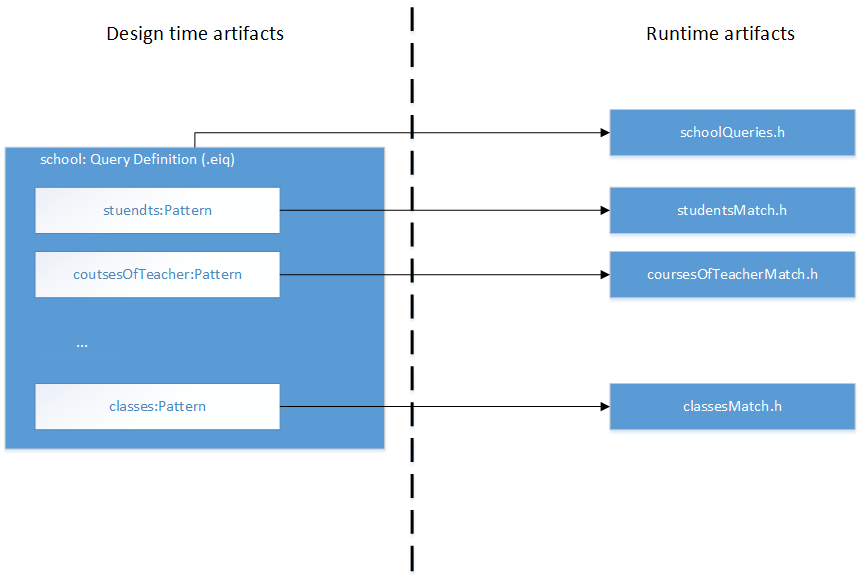
\includegraphics[width=120mm, keepaspectratio]{figures/iterator_gen_art.png}
\caption{The generated artifacts for the iterator based approach}
\label{fig:iter_gen_art}
\end{figure}

As the image shows, the generated artifacts are similar to the runtime based
approach. There is a single header file generated for each query definition
file and one-one additional header for each pattern. The difference is that it
is not necessary to generate the frames, as the variables the runtime stored in
the frame are held in local variables using this approach. This might suggest
that the generated code complexity got reduced, but the exact opposite is true
as listing \listref{tos_gen_iter} illustrates.

\begin{lstlisting}[frame=single,float=!ht,language=C++,
label=listing:tos_gen_iter, caption=Segment of the generated code for
teachers of school]

for(auto&& school : (::school::school::School::_instances)) {
	for(auto&& teacher : school->teachers) {
		if(_classHelper->is_super_type(teacher->get_type_id(), Teacher::type_id)) { 
			<assemble match> 
		}
	}
}

\end{lstlisting}

This code segment does exactly the same as the one shown for the runtime. In
this case, the code might even seem shorter, but as the queries grow larger the
code gets a lot more convoluted, for example when the search plan consists of
tens or even hundreds of steps, it gets hard to determine what the if statement
in the middle of the plan does, meanwhile in the case of the runtime based
approach, it will still be obvious as the method name itself tells what the
operation does. 

The above mentioned negatives of this approach are negligible, since the human
readability of a generated code is usually not important. For a release build,
it is always better to use this approach, as it is faster because there is no
need to check which operation is next from a search plan and the compiler can
generate more efficient bytecode since it is far easier to optimize this
version. In addition, the readability of this version could be improved through
annotating the code with comments describing which search operation gets
executed.

\subsection{Binding variables}\label{sect:binding_variables}

As previously mentioned, it is possible to bind variables of a pattern before
executing the query. This means that it is possible to predetermine the value of
a pattern variable, thus reducing the resulting matches to those that have the
predefined value in the specific variable. This is mostly useful if the query
can start from a predefined element of a model, significantly reducing the
pattern complexity.

The variable bindings have to be defined during query development time. The
generated code will adapt to the defined bindings and generate methods with the
specified parameters for a query. Listing \listref{pattern_binding} shows an
example of binding a parameter for a pattern.

\begin{lstlisting}[frame=single,float=!ht,language=IQPL,
label=listing:pattern_binding, caption=Binding of a parameter]

@Bind(parameters={teacher})
pattern classesOfTeacher(teacher, schoolClass) {
	find coursesOfTeacher(course, teacher);
	Course.schoolClass(course, schoolClass);
}

\end{lstlisting}

The parameter binding is done through the \emph{@Bind} annotation, where the
parameters have to be specified. It is possible to define multiple variables by
enumerating them using comma as a separator. The example binds the
\emph{classesOfTeacher} patterns \emph{teacher} parameter. That means a method
gets generated with a Teacher instance as a parameter which has to be specified.

\chapter{Localsearch Runtime}
\section{EMF to \CPP{} generation} \label{sect:CppObjectModel}

This chapter focuses on the ECore metamodel used to describe the class hierarchy
of the generated code and the structure of the generated code. This chapter also
discusses several issues related to the usage of \CPP{} and their solutions.

%----------------------------------------------------------------------------
\subsection{Metamodel}\label{sec:Metamodel}
%----------------------------------------------------------------------------

\begin{figure}[!ht]
\centering
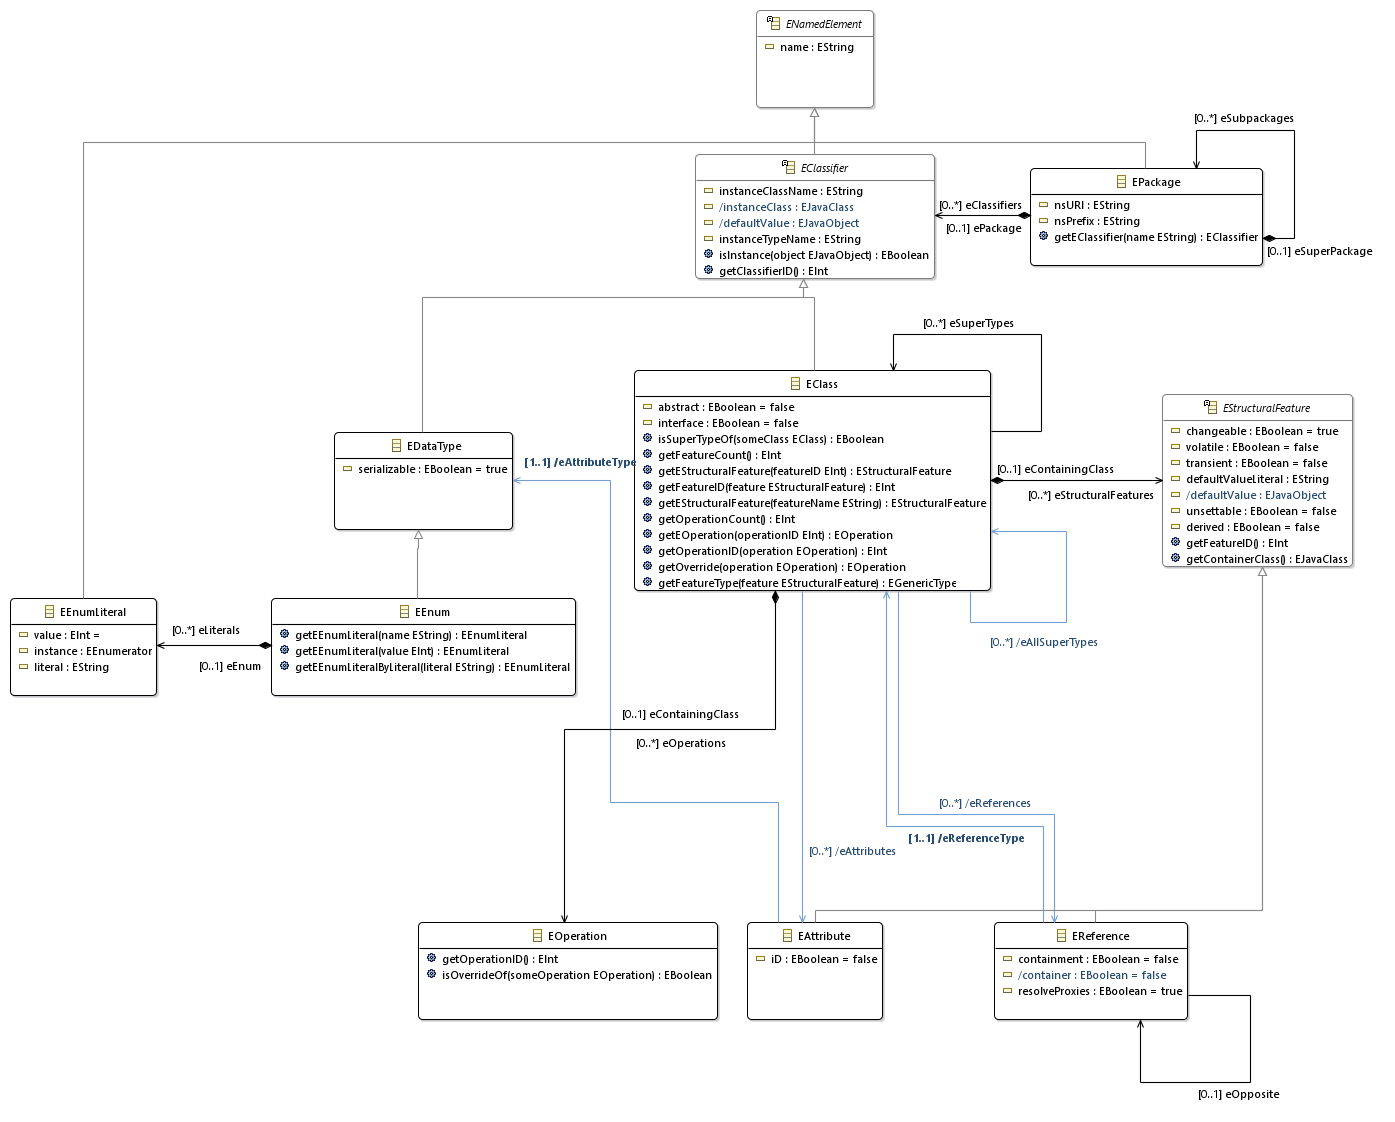
\includegraphics[width=145mm, keepaspectratio]{figures/ecore_diagram.png}
\caption{The ECore Class diagram metamodel.}
\label{fig:metamodel}
\end{figure}

The metamodel (as seen on figure \figref{metamodel}) is a simplified version of
an UML class diagram. The root of it is \emph{Model} that can contain
definitions of \emph{PrimitiveType}s and \emph{Package}s. Primitive types are
types native to a language like \emph{int}, \emph{string} etc. Packages allow
the classes to be structured in a hierarchical manner. Every package can contain
other packages or \emph{UMLClass}es. An UMLClass may contain
\emph{Relationship}s and \emph{Argument}s. A relationship can be either
\emph{Association} or \emph{Generalization}, of which a generalization
symbolizes inheritance while an association means the classes refer to each
other. A generalization refers to it's super UMLClass, while an association has
a source and a target UMLClass. Arguments are values of specified primitive
types. Arguments and associations inherits from \emph{MultiplicityElement}, this
allows their multiplicity to be specified (e.g. [0..1], [0..*]). Most elements
of the model inherit from \emph{NamedElement}, this gives them a string
\emph{name} identifier. This model allows for the creation of basic class
diagrams that support most necessary features.

%----------------------------------------------------------------------------
\subsection{Generated code structure}\label{sect:GeneratedCodeStructure}
%----------------------------------------------------------------------------

To talk about the generated code structure, it is necessary to have an actual
class diagram for example, this class diagram is shown on figure
\figref{InstanceModel}.

\begin{figure}[!ht]
\centering
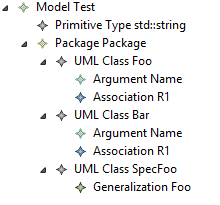
\includegraphics[width=65mm, keepaspectratio]{figures/instance_model.png}
\caption{An example class diagram.}
\label{fig:InstanceModel}
\end{figure}

The model defines one primitive type, which is the \CPP{} \emph{string}. It has
a single package \emph{Test}, which contains all the classes. Classes \emph{Foo}
and \emph{Bar} both have a \emph{Name} attribute and an \emph{R1} association
between them. The class \emph{SpecFoo} inherits from \emph{Foo}.

The structure of the generated code can be seen on figure
\figref{GenCodeStruct}.

\begin{figure}[!ht]
\centering
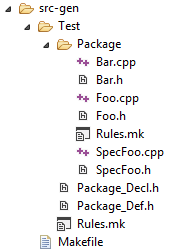
\includegraphics[width=40mm, keepaspectratio]{figures/gen_code_struct.png}
\caption{The generated code structure.}
\label{fig:GenCodeStruct}
\end{figure}

The model get generated into a folder named accordingly inside the src-gen
folder of the project. For every package a folder and two header files are
created. The \emph{def} header file contains includes to classes inside the
package, while the \emph{def} header contains the one liner definitions of said
classes. The folder created for the package contains header and source files for
each class and, if there are any, the above explained files for packages. To
help with compilation, a makefile also gets generated. The root folder has the
makefile itself, which then includes the rule files in the folders recursively.
This way the users only job is to create the main file and the code can be
easily compiled. Another way to use the generated code would be to simply
include the rule file in the user's own make file in another project. This gives
great flexibility to anyone using a make based build tool.

\section{Runtime Library}

This section will mostly focus on the implementation specific details of the
\CPP{} localsearch runtime, such as problems specific to \CPP{} and their
solutions, the structure of a search plan, it's operations and their execution.

%----------------------------------------------------------------------------
\subsection{\CPP{} specific problems}\label{sect:CppSpecificProblems}
%----------------------------------------------------------------------------

In the case of the runtime, \CPP{} brought with it's speed several problems, such
as the lack of any reflection api and a unified object base class. This caused
several issuses during the implementation, because running localsearch over \CPP{}
objects requires instance checking, getting fields by name to navigate
associations and iterating over every instance of a specific task. This section
will propose a solution for each of the above mentioned issues.

%----------------------------------------------------------------------------
\subsubsection{Objects in \CPP{}}\label{sect:ObjectsInCpp}
%----------------------------------------------------------------------------

During the localsearch process it is necessary to hold every single object in
containers without knowing their type. In \CPP{} there are three main ways to do
this.

\begin{itemize}
  \item using heterogeneous collections with a common base class
  \item \emph{void*} pointer
  \item wrapper object
  \item using templates
\end{itemize}

Using a common base class is probably the easiest and most obvious solution,
but it would constraints the type of objects the local search runtime can
be used on which makes this solution undesireable.

Using \emph{void*} pointers would mean the complete loss of type information,
thus making any dynamic type checking mostly impossible. This alone makes this
solution unusable.

The third method of using wrapper object is a possible solution with the
only drawbacks of being complicated, slow and memory inefficient.

The last, template based version is probably the most complicated one. It
requires complicated template programming which results in slower compile times
and larger executables, but it has a superior runtime speed and memory usage to
all other alternatives.

\textbf{Wrapper object based solution}

 The structure of the warpper object can be seen on figure
 \ref{fig:wrapper_structure}.

\begin{figure}[!ht]
\centering
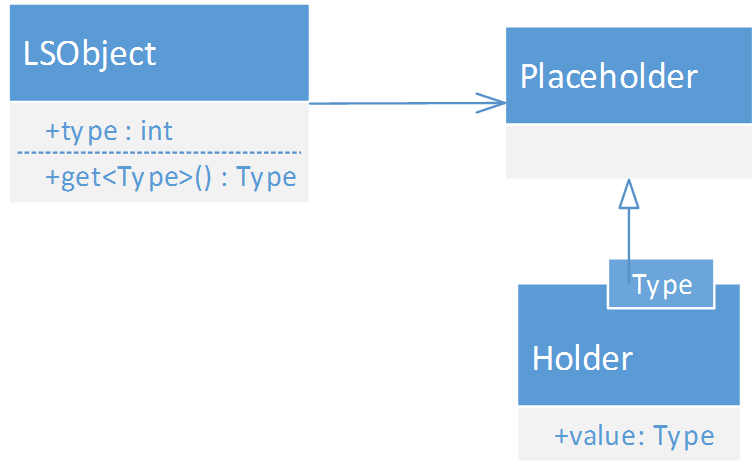
\includegraphics[width=70mm, keepaspectratio]{figures/wrapper_structure.png}
\caption{The structure of the wrapper object.}
\label{fig:wrapper_structure}
\end{figure}

The \emph{LSObject} (Local Search Object) contains the type information, a
template method to get the value contained cast to the proper type and a pointer to a
\emph{Placeholder} object. The actual object contained is actually of the
\emph{Holder} template type, which contains the original value. The placeholder
object's construction can be seen as below.

\begin{lstlisting}[frame=single,float=!ht,language=C++, caption=Constructing a
wrapper object.] template<typename T>
LSObject(const T& value, int type) :
	_ptr(new Holder<T>(value)), type(type) {
}
\end{lstlisting}

As it can be seen from the code, the \emph{LSObject}'s holder will hold a
reference to the value, be it pointer or actual value. The second parameter
\emph{type} contains the type information for the value. 

\begin{lstlisting}[frame=single,float=!ht,language=C++, caption=Retrieving
correctly typed object.]
template<typename T>
inline T& LSObject::get() const {
    return static_cast<Holder<T>&>(*this->_ptr).value;
}
\end{lstlisting}


The \emph{get} method of the wrapper object returns the value as it was passed
in, however this require the compile time knowledge of the original type. The
implementation can be seen below:

The usage of the wrapper class is shown in listing \listref{wrapper_usage}.

\begin{lstlisting}[frame=single,float=!ht,language=C++,
label=listing:wrapper_usage, caption=Wrapper object usage.]
Foo f;
f.Name = "Foo1";
LSObject ls_f(f, 0);

ls_f.get<Foo>().Name
\end{lstlisting}

The design of the class was heavily inspired by the \emph{boost::any} class.

The main problem with this approach is it's speed. The speed issue is caused by
the fact that while iterating over the instances of a class, they all have to be
wrapped in a wrapper class while creating a new collection. This costs a
considerable amount of time. Also for this reason, the memory footprint of this
solution is considerably higher.

\textbf{Template based solution}

This solution needed the most effort in implementation, since this requires
the type information to flow through the whole runtime. The main idea of the
solution is that all components of the engine have several template parameters
to describe the types it has to handle. The listing \listref{template_example}
contains the declaration of a navigation class, which shows how complicated
class declarations can get using this approach.

\begin{lstlisting}[frame=single,float=!ht,language=C++,
label=listing:template_example, caption=Template based approach example.]
template<typename SrcType, typename TrgType, typename Collection, 
		typename Member, typename MatchingFrame>
class NavigateMultiAssociation
  : public ExtendOperation<TrgType, Collection, MatchingFrame>;
\end{lstlisting}

The main benefits of this solution are speed and really low memory usage. The
speed is gained from the fact that, with this approach, iterators can be used
over the original instances collections without any wrapping, and only
filtering is necessary. This also means that the memory usage scales with
pattern complexity and is completely independent of model size.

%----------------------------------------------------------------------------
\subsubsection{Iterating class instances}\label{sect:IteratingClassInstances}
%----------------------------------------------------------------------------

To allow iteration over all instances of a class, a registry needs to be managed
which gets updated on each instance construction or deletion. The only feasible
way to do this is to write the classes constructor and destructor in a way that
it adds new instances to a list when they are created and removes them when they
are deleted. This method limits the type of objects the runtime works on, but
this is the most reasonable solution. An example of a class prepared to count
its instances can be seen below.

\begin{lstlisting}[frame=single,float=!ht,language=C++]
class Foo  {
public:
	Foo() {
		_instances.push_back(this);
	}
	
	~Foo() {
		_instances.remove(this);
	}
		
	static std::list<Foo*> _instances;
};
\end{lstlisting}

This solution uses the \emph{std::vector} to contain the created instances.
While the constructor is trivial the destructor is more interesting. The
check whether the destructed object is in the vector seems unnecessary, but \CPP{}
allows the allocation of memory for an object without actually calling it's
constructor. This memory portion can be freed with delete which also calls the
destructor. In this case, the instance will not be in the vector and this could
cause issues.

%----------------------------------------------------------------------------
\subsubsection{Instance checking}\label{sect:InstanceChecking}
%----------------------------------------------------------------------------

In the case of \CPP{} the generally accepted way of dynamic type checking is using
\emph{dynamic\textunderscore cast} provided by the language. This is hovewer a
not ideal solution. The first problem is it only works on dynamic classes, i.e.\
classes with at least one virtual method. The other issue is speed, as
\emph{dynamic\textunderscore cast} uses vtables to check if the specified
instance can be casted to the specified type. To illustrate the speed issues,
the following table (\ref{tab:InstPerf}) shows the results of performance tests
made in \CPP{} and Java.

\begin{table}[ht]
	\footnotesize
	\centering
	\caption{Instance of check performance comparison of Java and \CPP{}}\label{tab:InstPerf}
	\begin{tabular}{ | l | c | c |}
	\hline
	Iterations 	& Java 		& \CPP{} 		 \\ \hline
	$10^4$ 		&  1	ms 	& 0.1	ms \\
	$10^5$ 		&  11 	ms  & 1		ms \\
	$10^6$ 		&  15 	ms  & 17	ms \\
	$10^7$ 		&  41 	ms  & 173	ms \\
	$10^8$ 		&  261 	ms  & 1746	ms \\
	$10^9$ 		&  2515 ms  & 17456	ms \\
	\hline
	\end{tabular}
	\label{tab:TabularExample}
\end{table}

As the table shows, java is slower on small number of iterations, but on higher
number of iterations the JIT compiler manages to optimize the instance checking
process and gets roughly a magnitude faster than \CPP{}.

The solution I propose is an inheritance matrix in which it is contained whether
an instance of a type is a child of another type. This can be generated using
the model of the classes. This also means that most of the calculation is done
generation time, thus making this method faster than most dynamic type
inference method provided by languages. For the following examples I will use
the class structure shown on figure \ref{fig:simple_class} . In this example
there are three classes, \emph{Foo}, \emph{Bar} and \emph{SpecFoo}.
\emph{SpecFoo} extends \emph{Foo}. The example does not contain any of
the possible more complex hierarchy structures, like diamond, but nonetheless it
supports them.

\begin{figure}[!ht]
\centering
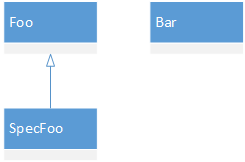
\includegraphics[width=50mm, keepaspectratio]{figures/simple_class.png}
\caption{Example class structure.}
\label{fig:simple_class}
\end{figure}

To use this method, the runtime knowledge of a classes exact instance is
required. This could be done via a virtual method (which is undesireable
because of larger memory footprint for instances) or template metaprogramming.
Template metaprogramming would only work on the static type of the object, not
the dynamic, i.e. it would not work correctly with inheritance. For example for
the pointer \emph{Foo* f = new SpecFoo()} it would always return Foo as the
type, same with the built in \emph{\texttt{type\_id}} function. Thus the only
viable solution in my case is the virtual method. An implementation example for
such solution can be seen in the following example (expanding uppon the
previous code sample):

\begin{lstlisting}[frame=single,language=C++, label=listing:type_id,
caption=Type identifier for classes.]
class Foo  {
public:
	Foo() {
		_instances.push_back(this);
	}
	
	~Foo() {
		_instances.remove(this);
	}
	
	virtual unsigned short get_type_id() const {
        return type_id;
    }
		
	static std::list<Foo*> _instances;
	static const unsigned short type_id = 1;
};
\end{lstlisting}

In this example, the \emph{\texttt{type\_id}} is generated. This might cause
issues if the code is generated in multiple sessions. This can be solved with a
class that has a growing id for each of it's instance, and a bit of template
metaprogramming. A simplified solution can be seen below:

\begin{lstlisting}[frame=single,float=!ht,language=C++,
label=listing:unique_number, caption=Unique number generation for type
identifiers.]
class unique_number { 
public:
	unique_number(): cur_id(max_id++) {}

private:
	static unsigned long max_id;
	unsigned long cur_id;
};

template<typename C>
struct type_number {
	static unique_number number;
};

class Foo  {
	...
	
	virtual unsigned short get_type_id() const {
        return type_number<Foo>::number;
    }
    
	...
};
\end{lstlisting}

The basic idea is that every instance of \emph{\texttt{unique\_number}} contains
a unique identifier. For each class, a separate \emph{\texttt{type\_number}}
gets created compile time with a \emph{\texttt{unique\_number}} inside, which can be
retrieved in the \emph{\texttt{get\_type\_id}} method. This guarantees a unique
id for each class that's calculated compile time.

Using this type id as an identifier it is possible to create a boolean matrix
(two dimensional array) of the type relationships. For each member of this matrix
'm' 
\[
m[type1][type2] = type1\textrm{ instanceof }type2
\]

In the case of the presented example this matrix would look like in the
following table (\ref{tab:InhMatrix}):

\begin{table}[ht]
	\footnotesize
	\centering
	\caption{Example inheritance matrix}\label{tab:InhMatrix}
	\begin{tabular}{| c | c | c | c |}
	\hline
			& Foo	& Bar	& SpecFoo	\\ \hline
	Foo		& true	& false	& false		\\ \hline
	Bar		& false	& true	& false		\\ \hline
	SpecFoo	& true	& false	& true		\\ \hline
	
	\hline
	\end{tabular}
	\label{tab:TabularExample}
\end{table}

The diagonal of the matrix is obviously true (since an instance of Foo is
trivially the instance of Foo). The SpecFoo instance is the instance of both Foo
and SpecFoo.

This method allows instance checking to be done in basically two array indexing
operations. From my performance measurements, this method seem to be marginally
faster than the java \emph{instanceof} operation.

\begin{table}[ht]
	\footnotesize
	\centering
	\caption{Instance of check performance comparison of Java,
	\CPP{} and inheritance matrix}\label{tab:InstPerf}
	\begin{tabular}{ | l | c | c | c |}
	\hline
	Iterations 	& Java 		& \CPP{}	&	Inheritance Matrix	\\ \hline
	$10^4$ 		&  1	ms 	& 0.1	ms	&	0.03	ms			\\
	$10^5$ 		&  11 	ms  & 1		ms	&	0.3		ms			\\
	$10^6$ 		&  15 	ms  & 17	ms	&	3		ms			\\
	$10^7$ 		&  41 	ms  & 173	ms	&	15		ms			\\
	$10^8$ 		&  261 	ms  & 1746	ms	&	172		ms			\\
	$10^9$ 		&  2515 ms  & 17456	ms	&	1725	ms			\\
	\hline
	\end{tabular}
	\label{tab:TabularExample}
\end{table}

%----------------------------------------------------------------------------
\subsubsection{Navigation through associations}
\label{sect:NavigationThroughAssociations}
%----------------------------------------------------------------------------

Navigation through associations specified by their name requires meta
information about the classes. This information can be accessed using the \CPP{}
feature called \emph{pointer to member}. A pointer to member is similar to a
function pointer in that they allow the calling of a member function without
knowing its name. Yet, unlike ordinary an ordinary pointer to function, it also
enables the manipulation of data members of an object.

The following listing (\listref{p2m_decl}) shows an example of a pointer to
member declaration. In this case, a pointer to a member of the \emph{Teacher}
class is declared, which member has a \emph{std::string} type.

\begin{lstlisting}[frame=single,float=!ht,language=C++,
label=listing:p2m_decl, caption=Pointer to member declaration]
std::string Teacher::*name;
\end{lstlisting}

A pointer to member can be initialized to any member of the declared class with
the declared type. Listing \listref{p2m_init} shows how to do so.

\begin{lstlisting}[frame=single,float=!ht,language=C++,
label=listing:p2m_init, caption=Pointer to member initialization]
std::string Teacher::*name = &Teacher::name;
\end{lstlisting}

This pointer to member can be passed around to functions as parameter. With
this, it is easy to implement a simple method which navigates over an
association for any class. An example of such a method is shown in listing
\listref{p2m_usage}.

\begin{lstlisting}[frame=single,float=!ht,language=C++,
label=listing:p2m_usage, caption=An universal navigation method using pointer
to member] 
template<SrcType, TrgType, Member>
TrgType navigate(SrcType src, TrgType Member::* navigator) {
  return src->*navigator;
}
\end{lstlisting}

In this example, it is assumed that \emph{Member} and \emph{SrcType} is the
same. In a more realistic use case, the variable \emph{src} has to be casted to
either \emph{Member} or \emph{Member*} depending on weather \emph{SrcType} was a
pointer or value (which can be determined through template metaprogramming).

%----------------------------------------------------------------------------
\subsubsection{Missing value representation}
\label{sect:MissingValueRepresentation}
%----------------------------------------------------------------------------

The query api uses Match class instances to represent the query results. These
classes are basictly tuples which contain all the data related to a query
result. As the api supports querying of a single arbitrary match, it is
necessary to represent a missing value. This could be done using nullptr, but
that would require the result object to be a pointer, which means it has to be
dynamically allocated on the memory. This should be avoided, so another solution
was necessary.

The most common approach of representing a missing value is the null object
pattern. For this puprose, the runtime library contains an \emph{Optional}
class, which represents either a value or the absence of a value.

Listing \listref{optional} shows the interface of the optional class. An
optional instance can be requested through static methods, for either a missing
value or a present value. The \emph{get} method allows the retrieval of the
value or throws an error if the value is missing. It is possible to check for
the presence of a value through the \emph{present} method. There are additional
utility methods to handle the presence or absence of a value in a functional
style.

\begin{lstlisting}[frame=single,float=!ht,language=C++,label=listing:optional,
caption=Optional interface] 
template<typename T>
class Optional {
public:
        static Optional<T> empty();
        static Optional<T> of(T object);

        bool present();
        void if_present(void (*fun)(T));
        T or_else(T (*fun)());
        T or_else(T other);
        T get();
};
\end{lstlisting}

%----------------------------------------------------------------------------
\subsection{Library Architecture}\label{sect:Runtime_library}
%----------------------------------------------------------------------------

The runtime library contains several classes to facilitate the running of
queries over \CPP{} object hierarchies. A simplified version of the library
class diagram can be seen on figure \figref{runtime}.

\begin{figure}[!ht]
\centering
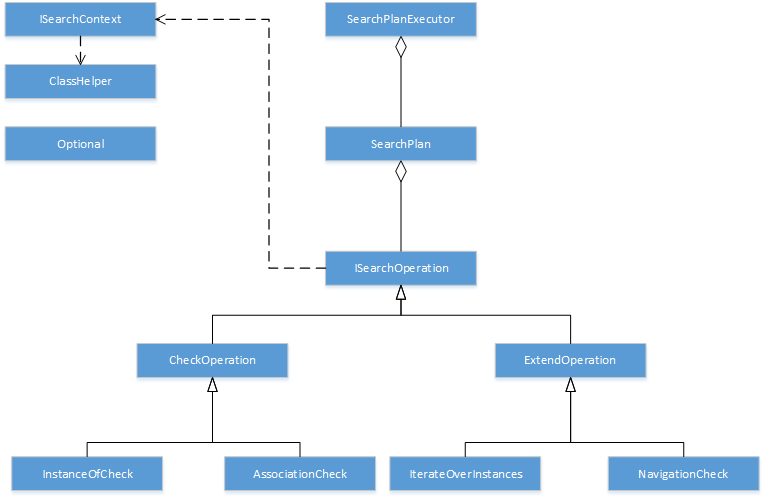
\includegraphics[width=150mm, keepaspectratio]{figures/runtime_diagram.png}
\caption{The runtime library.}
\label{fig:runtime}
\end{figure}

The runtime library consists of three utility classes. The \emph{ISearchContext}
is the context of a search operation. It gives access to other utility class
instances parametrized correctly for the current search operations context. Such
utility class is the \emph{ClassHelper} which contains the dynamic instance
checking functionality described in section \sectref{InstanceChecking}. Another
utility class is \emph{Optional}, its purpose is detailed in
\sectref{MissingValueRepresentation}.

The rest of the library deals with the execution of a search plan. The central
piece of these classes is \emph{SearchPlan}. It contains an ordered list of
\emph{ISearchOperations}. An ISearchOperation can either be:

\begin{itemize}
  \item \emph{Check operation} - these type of operations recieve one or more
  value and determines if a constraint is satisfied by them.
  \item \emph{Extend operation} - these operations recieve zero or more values
  and based on those values calculates an additional value.
\end{itemize}

A check operation can either be an \emph{InstanceOfCheck} or an
\emph{AssociationCheck}. The InstanceOfCheck tests wether the provided value is
of the expected type. This is done as explained previously
(\sectref{InstanceChecking}). The AssociationCheck tests wether two values are
related through an association. This has two cases, if the association is [0..1]
multiplicity, this is a simple equality check, while if the association is
[0..*] then this is a list containment check.

Similarly to a check operation, the extend operation has two main types:
\emph{IterateOverInstances} and \emph{NavigateAssociation}. IterateOverInstances
simply assigns all instances of a class to a variable one by one.
NavigateAssociation gets a value and an association as a parameter and assigns
the instance or instances reached by navigating the association from the given
value to a variable.

The search plan is executed with the help of the \emph{SearchPlanExecutor}. The
search plan executor simply executes the search operations of a search plan and
returns if a match is found. This also provides an iterator with which a search
plan can be executed in a lazy manner.

\section{Generated code and API}\label{sect:generated_code_and_api}

The patterns defined with the \EIQ{} Pattern Language can be executed through
the usage of the generated classes. This chapter section goes into detail
explaining the generated classes.

The program supports two different approaches for executing the queries in the
generated code: \emph{runtime} based and \emph{iterator} based. The runtime
based fully utilizes the previously showcased local search runtime, assembles a
search plan and executes it. Meanwhile, the iterator based approach only uses a
few parts of the runtime and mostly uses built in language constructs.

\subsection{Runtime based}

This approach uses all the available runtime classes to generate a mostly easy
to understand human readable generated code where the search operations are
clearly visible. 

The generated artifacts for the runtime based approach can be seen on figure
\figref{runtime_gen}. The runtime based approach generates one header file per
query definition file and two header files for each pattern definition. 

\begin{figure}[!ht]
\centering
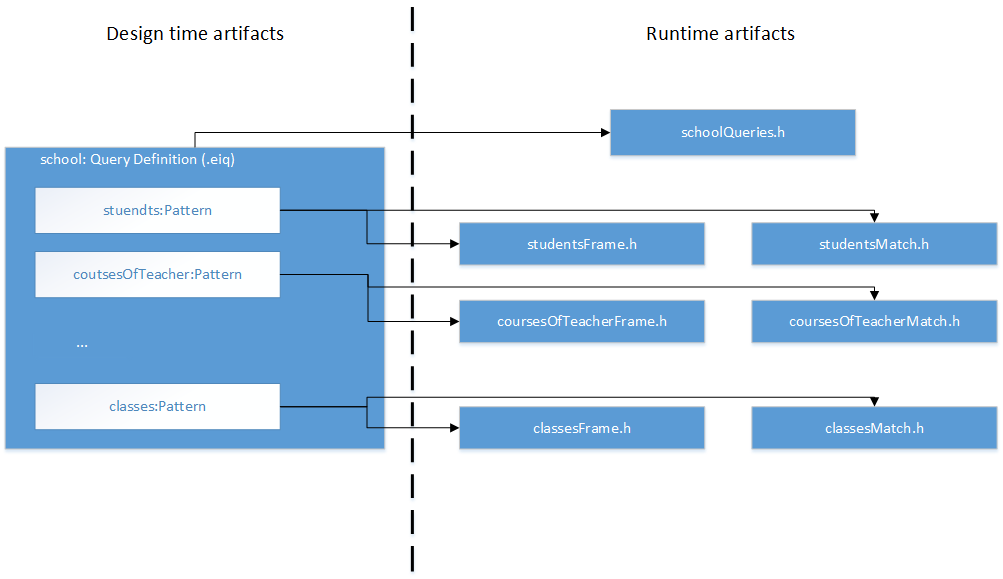
\includegraphics[width=130mm, keepaspectratio]{figures/runtime_gen_art.png}
\caption{The generated artifacts for the runtime based approach}
\label{fig:runtime_gen}
\end{figure}

The single central header file generated for a query definition file is named
after the original with the following pattern: \emph{<original .eiq name>Queries.h}.
Its function is to provide an API to call the defined patterns in multiple
ways:

\begin{itemize}
  \item \emph{get\_all\_<pattern>} - retrieves all matches for the defined pattern.
  \item \emph{get\_one\_<pattern>} - returns a single, arbitrary match for
  the defined pattern.
\end{itemize}

These methods also get generated with different parameter lists based on the
defined pattern bindings. More information about pattern bindings will be
explained in section \sectref{binding_variables}. In addition, it also contains
the initialization of the inheritance matrix which is generated from the
metamodel.

The two headers generated for a single pattern are representing a related
\emph{Frame} and a \emph{Match}. The frame is only used internally, it is a
simple struct containing all the variables used during the process of
executing the local search algorithm. The match represents a single match of the
pattern, it contains all the variables defined by the user as external variable
(defined in the patterns parameter list and not in the body).

To illustrate how the generated code is easy to understand, listing
\listref{tos_gen_runtime} shows the generated code for the
\emph{teachersOfSchool} pattern (reminder of the pattern in listing
\listref{tos_pattern_rem}). As seen in the code, the search plan is assembled
one operation at a time, while the operations are named in a way that it is easy
to understand what it will do. 

\begin{lstlisting}[frame=single,float=!ht,language=IQPL,
label=listing:tos_pattern_rem, caption=Teachers of school pattern as a
reminder] 
pattern teachersOfSchool(teacher, school) {
	School.teachers(school, teacher); 
}
\end{lstlisting}

In this example, the first operation is an instance iteration, where each
instance will be assigned to the first slot of the frame, and the iterated
instances are of the School class. The second operation navigates through a
School instance's teachers association and the found Teacher instances get
stored in the frames zeroth slot. Then as a third operation, the search checks if the
zeroth slot in the frame is of the Teacher type. This check seems unnecessary
and it is in this case, but if the School's teachers association pointed to a
parent type of Teacher, than the check would be required to filter out invalid
matches. This is a point in which the generated search plan could be further
optimized.

\begin{lstlisting}[frame=single,float=!ht,language=C++,
label=listing:tos_gen_runtime, caption=Segment of the generated code for
teachers of school]

SearchPlan< TeachersOfSchoolFrame> sp;
		
sp.add_operation(create_IterateOverInstances(&TeachersOfSchoolFrame::_1,
				School::type_id));
sp.add_operation(create_NavigateMultiAssociation(&TeachersOfSchoolFrame::_1,
				&TeachersOfSchoolFrame::_0,
				&School::teachers));
sp.add_operation(create_InstanceOfCheck(&TeachersOfSchoolFrame::_0,
				Teacher::type_id));

\end{lstlisting}


\subsection{Iterator based}

The iterator based approach is a much simpler approach than the runtime based
one, as it mostly uses built in language constructs and standard library
iterators. The main reason for this approach is that it reduses the dependency
on the runtime and it is slightly faster than the runtime based approach, but
the code readability is a lot worse and the generated code amount is much
larger. The generated artifacts are shown on figure \figref{iter_gen_art}.

\begin{figure}[!ht]
\centering
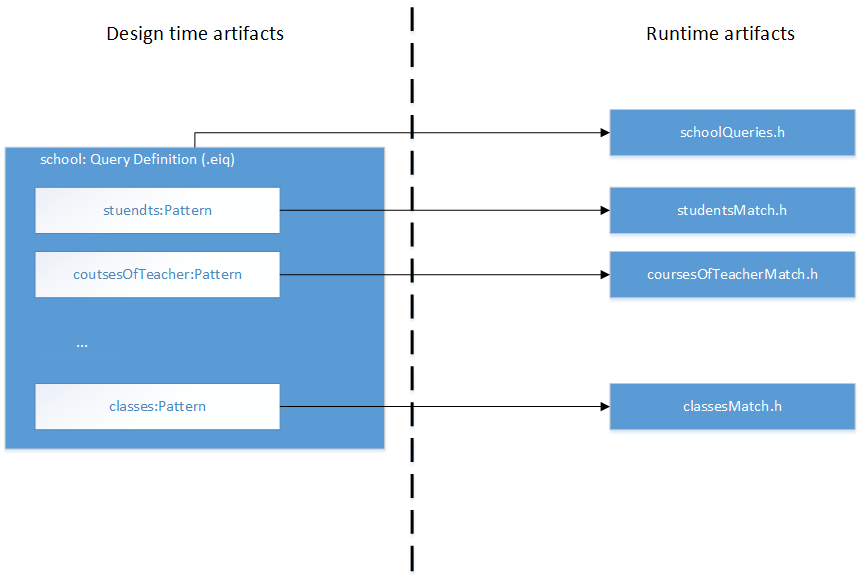
\includegraphics[width=120mm, keepaspectratio]{figures/iterator_gen_art.png}
\caption{The generated artifacts for the iterator based approach}
\label{fig:iter_gen_art}
\end{figure}

As the image shows, the generated artifacts are similar to the runtime based
approach. There is a single header file generated for each query definition
file and one-one additional header for each pattern. The difference is that it
is not necessary to generate the frames, as the variables the runtime stored in
the frame are held in local variables using this approach. This might suggest
that the generated code complexity got reduced, but the exact opposite is true
as listing \listref{tos_gen_iter} illustrates.

\begin{lstlisting}[frame=single,float=!ht,language=C++,
label=listing:tos_gen_iter, caption=Segment of the generated code for
teachers of school]

for(auto&& school : (::school::school::School::_instances)) {
	for(auto&& teacher : school->teachers) {
		if(_classHelper->is_super_type(teacher->get_type_id(), Teacher::type_id)) { 
			<assemble match> 
		}
	}
}

\end{lstlisting}

This code segment does exactly the same as the one shown for the runtime. In
this case, the code might even seem shorter, but as the queries grow larger the
code gets a lot more convoluted, for example when the search plan consists of
tens or even hundreds of steps, it gets hard to determine what the if statment
in the middle of the plan does, meanwhile in the case of the runtime based
approach, it will still be obvious as the method name itself tells what the
operation does. 

The above mentioned negatives of this approach are negligable, since the human
readability of a generated code is usually not important. For a release build,
it is always better to use this approach, as it is faster because there is no
need to check which operation is next from a search plan and the compiler can
generate more efficient bytecode since it is far easier to optimize this
version. In addition, the readability of this version could be improved through
annotating the code with comments describing which search operation gets
executed.

\subsection{Binding variables}\label{sect:binding_variables}

As previously mentioned, it is possible to bind variables of a pattern before
executing the query. This means that it is possible to predetermine the value of
a pattern variable, thus reducing the resulting matches to those that have the
predefined value in the specific variable. This is mostly useful if the query
can start from a predefined element of a model, significantly reducing the
pattern complexity.

The variable bindings have to be defined during query development time. The
generated code will adapt to the defined bindings and generate methods with the
specified parameters for a query. Listing \listref{pattern_binding} shows an
example of binding a parameter for a pattern.

\begin{lstlisting}[frame=single,float=!ht,language=IQPL,
label=listing:pattern_binding, caption=Binding of a parameter]

@Bind(parameters={teacher})
pattern classesOfTeacher(teacher, schoolClass) {
	find coursesOfTeacher(course, teacher);
	Course.schoolClass(course, schoolClass);
}

\end{lstlisting}

The parameter binding is done through the \emph{@Bind} annotation, where the
parameters have to be specified. It is possible to define multiple variables by
enumerating them using comma as a separator. The example binds the
\emph{classesOfTeacher} patterns \emph{teacher} parameter. That means a method
gets generated with a Teacher instance as a parameter which has to be specified.

\section{A practical example}

The aim of this section is to provide an example of the full workflow using the
created program throughout a realistic scenario. This section will show how to
use a predefined metamodel to write queries, generate model and query code, and
describes the usage of the generated code with a simple code example. This
example will use the previously defined \emph{school} metamodel
(\figref{School_Metamodel}). The example assumes an already created
eclipse modeling project with the metamodel inside it.

The first step of the workflow is determining the required queries and writing
them. The scenario is that the \CPP{} program requires a query to determine the
school a student goes to in an efficient manner. To do this, an \emph{.eiq} file
must be created in the project on the source path. The contents of the
\emph{.eiq} will be described in listing \listref{example_school_eiq}

\begin{lstlisting}[frame=single,float=!ht,language=IQPL,
label=listing:example_school_eiq, caption=The \emph{.eiq} file for the example
project] 
package hu.bme.mit.cpp.localsearch.school.query

import "http://school.ecore"

@Bind(parameters={student})
pattern studentsOfSchool(student, school) {
	Student.schoolClass.courses.school(student, school);
}
\end{lstlisting}

The \emph{.eiq} file contains a package declaration, an import to the metamodel
and a single pattern defining the required query. The query returns all
school-student pair where the student goes to the given school. The \emph{@Bind}
annotation defines that the student is a bound parameter, which means it can be
specified from the code so that the query will only search for the school.

The next step is generating the model and query code. The model code can be
generated via right clicking the \emph{.ecore} file describing the metamodel
and using the \emph{EMF Generator -> Generate \CPP{} files} option. This generates
the \CPP{} classes from the metamodel in the \emph{cpp-gen} folder. The query
code can be generated in similar fashion, by right clicking the \emph{.eiq} file
and selecting the appropriate option from the \emph{Generate query code\ldots}
menu. The available options is either runtime based or iterator based
implementation. For more on the differences of these generated code styles see
section \sectref{generated_code_and_api}.

The final step is the usage of the generated code. The code generator is
designed so that the \emph{cpp-gen} folder can be used as a project folder. The
model generator also generates a \emph{makefile} which can be used to build the
project with \emph{GNU Make}. The \emph{makefile} should work out of the box
most of the time, but if the runtime library is not installed inside the default
library and include paths for the system or is not next to the original modeling
project, some modifications might be required. The makefile defines the
\emph{CXXFLAGS} and \emph{LIBPATH} variables, these have to be modified to use
the proper runtime library path. If the makefile is properly configured, the
easiest way to use the generated code is by creating a \emph{main.cpp} file in
the \emph{cpp-gen} folder containing the user code. In this example the contents
of the \emph{main.cpp} file can be seen in listing \listref{example_school_cpp}

\begin{lstlisting}[frame=single,float=!ht,language=C++,
label=listing:example_school_cpp, caption=Fragment of the \emph{main.cpp}
file for the example project]

#include "school/school_def.h"
#include "Localsearch/school/schoolQueries.h"
// additional includes...

Student* initialize_model(); // implementation omitted

int main(int argc, char** args) {
	const Student* student = initialize_model();
	
	SchoolQueries engine;
	Optional<StudentsOfSchoolMatch> m = engine.get_one_students_of_school(student); 
	if(m.isPresent()) { 
		std::cout << "School of " 
				  << student.name << ": " 
				  << m.get().school.name <<	std::endl; 
	}
}
\end{lstlisting}

The example code uses \emph{\texttt{initialize\_model}} method to initialize the
model structure. It also returns the student whose school will be searched for.
The code then initializes the query engine and executes the query searching for
a single arbitrary school the student goes to. The returned value is an optional
of a match, which means the value might or might not be there. If there are no
matches to the query, then there is no result. Using the optional classes
\emph{isPresent()} method it is possible to determine wether a result was found.
If the result is present, then the code prints out the found school for the
student. The example code omits several include and using declaration and the
implementation of \emph{\texttt{initialize\_model}} method.

Building this code with running the \emph{make} command will result in an
executable which will initialize a model in the memory, execute a search on it
and print out the results.


\chapter{Scaleability and Performance}

One of the most important motivating factor for writing a \CPP{} implementation
of the local search runtime was performance. The assumption was that the \CPP{}
implementation, even though it might have many restrictions, would be
considerably faster than the original Java one. Several performance benchmarks
were done throughout the development to verify or deny the previous statement.

\section{Model}

The model used during the performance benchmarks was an instance of the
previously introduced school metamodel (figure \figref{School_Metamodel}).
Table \tabref{model_size} shows the model scales used during performance
benchmarking.

\begin{table}[ht]
	\footnotesize
	\centering
	\caption{Model size}\label{tab:model_size}
	\begin{tabular}{ | l | c | c | c | c | c | c |}
	\hline
	Scale	& Model Elements	& References	\\ \hline
	1 		&  2\,040			& 12\,633		\\
	2 		&  4\,080			& 25\,266		\\
	4		&  8\,160			& 50\,532		\\
	8		&  16\,320			& 101\,064		\\	
	16 		&  32\,640			& 202\,128		\\	
	32		&  65\,280			& 404\,256		\\	
	64 		&  130\,560			& 808\,512		\\	
	128 	&  261\,120			& 1\,617\,024	\\	
	256 	&  522\,240			& 3\,234\,048	\\	
	512		&  1\,044\,480		& 6\,468\,096	\\
	1\,024	&  2\,088\,960		& 12\,936\,192	\\	
	\hline
	\end{tabular}
	\label{tab:TabularExample}
\end{table}

The model size is defined with scale, which is essentially a simple multiplier
of the number of instances of each class defined in the metamodel. Larger
scales of a model simply created new instances of schools with similar
internal structure, but without any relationships not between the schools. The
instance model of a specified scale was generated using a deterministic
algorithm which was implemented in the same way in both Java and \CPP{},
allowing the comparison of the two framework implementation.

The measurements compare the performance of three implementations: Java Local
Search, Java RETE\cite{EIQ-Rete} and C++ iterator based. The Java Local Search
based implementation is the Java implementation of the local search algorithm
described in this thesis. The search plan generator is the same for both
the Java and \CPP{} Local Search solutions, but the Java implementation has
access to the model statistics which can influence the search plans. The Java
RETE algorithm based implementation is the default pattern matching
implementation used by \EIQ{}, which also means that this is the most mature of
the three approaches. It allows for incremental pattern matching, which
requires extensive caching which results in more memory usage and slower
initial search, but the cache is kept up to date internally through
notifications from the model, which means the second time a query is run it
will have a constant, very small return time.

\section{Performance measurements}

The first measurements focus on the time it takes to initialize and execute a
query on a model, retrieving every match. The first pattern is the really simple
\emph{students} pattern \listref{meas_students}, which retrieves matches every
student in the model. The main difficulty for this pattern is that the result
set is very large (more than 2 million elements for the largest scale), this
means the main bottleneck is the creation of the result set itself.

\begin{lstlisting}[frame=single,float=!ht,language=IQPL,
label=listing:meas_students, caption=The students pattern]
pattern students(student) {
	Student(student);
}
\end{lstlisting}

Figure \figref{meas_students} shows the execution times measured for each platform
with different implementations and on three model sizes: 256, 512 and 1024. Java
LS refers to the Java Local Search implementation, while the rest is self
explanatory.

\begin{figure}[!ht]
\centering
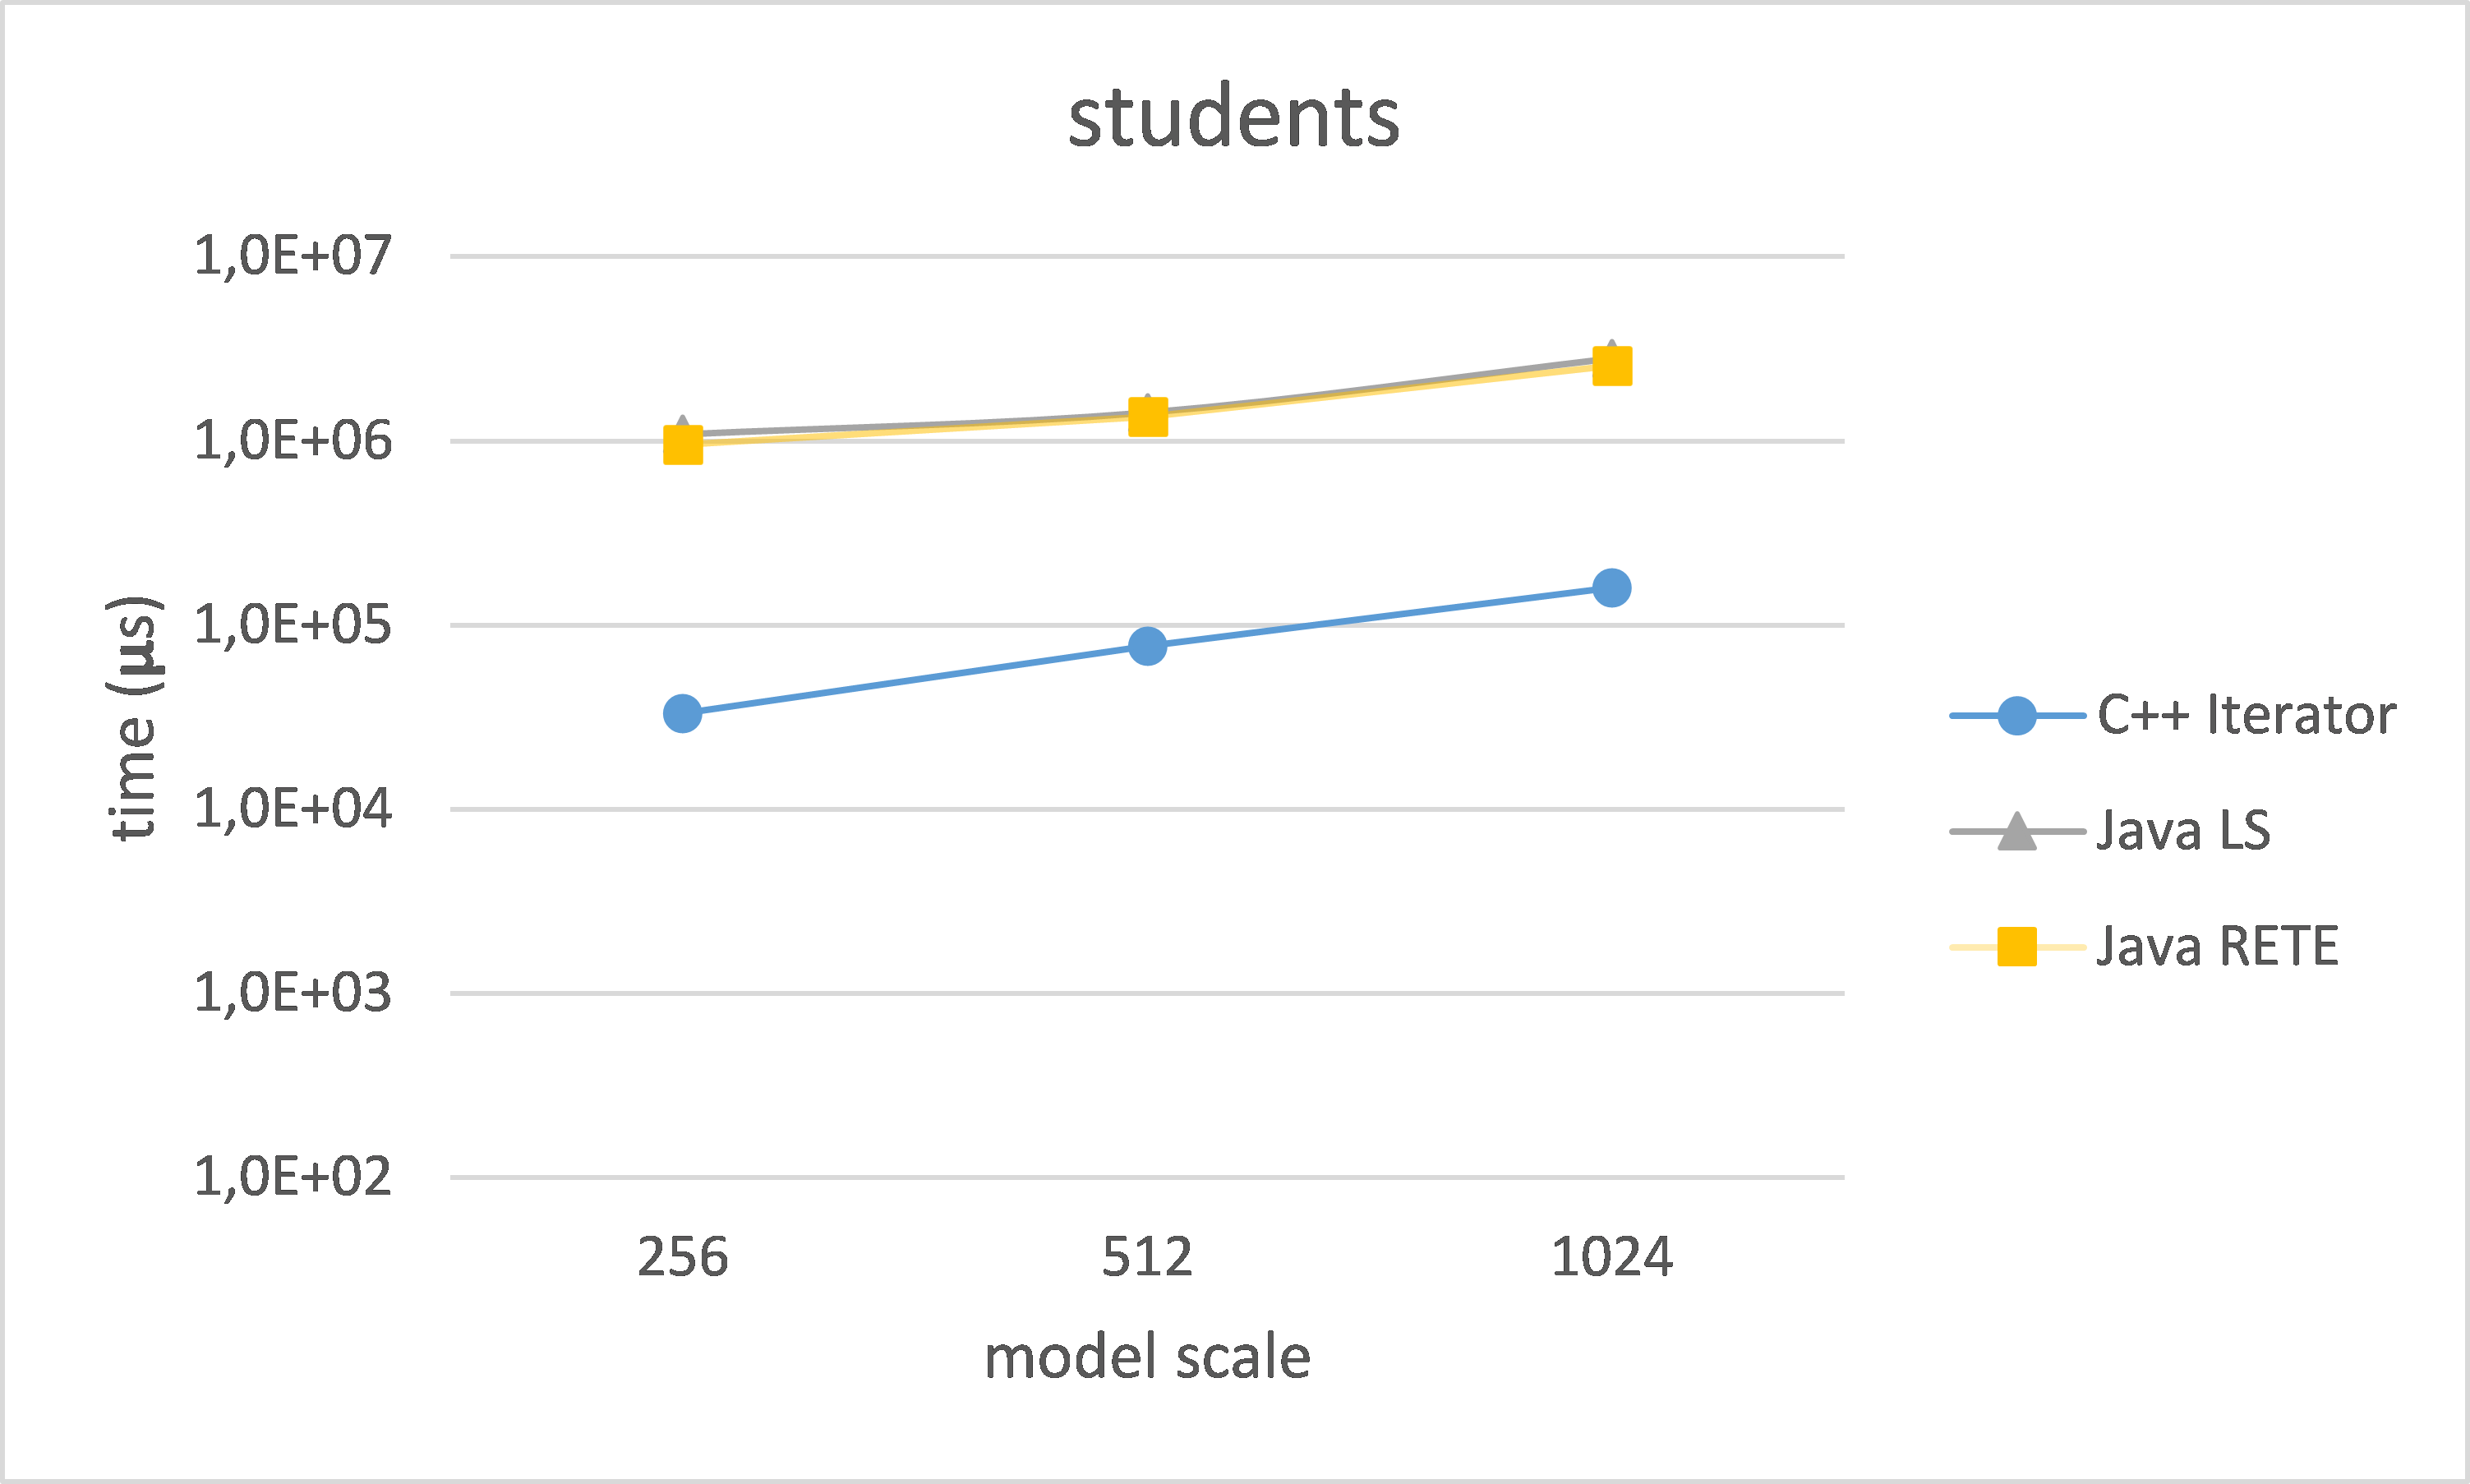
\includegraphics[width=120mm, keepaspectratio]{figures/meas_students.png}
\caption{Performance of the \emph{students} query}
\label{fig:meas_students}
\end{figure}

The measured times show the \CPP{} implementation performing considerably
better, then the Java ones. In the case of such a simple pattern this was
expected, as the \CPP{} implementation does a lot less preprocessing and most of
the query time consists of the assembly of the result set. The surprising part is
the fact the Java implementation of the local search algorithm does slightly
worse than the RETE based algorithm, which does a lot of advanced preprocessing and
caching. This could be the result of the immature codebase for the local search
based implementation, as it is still in development and might have optimization
issues.

The next examined pattern is the \emph{classesOfTeacher} pattern
(\listref{meas_classesOfTeacher}). This pattern is slightly more complex than
the previous one, however the result set is really small. The main takeaway from
this benchmark is how fast an implementation can respond to a very simple query
with only a few thousand matches.

\begin{lstlisting}[frame=single,float=!ht,language=IQPL,
label=listing:meas_classesOfTeacher, caption=The classesOfTeacher pattern]
pattern coursesOfTeacher(course, teacher) {
	Teacher.courses(teacher, course);
}

pattern classesOfTeacher(teacher, schoolClass) {
	find coursesOfTeacher(course, teacher);
	Course.schoolClass(course, schoolClass);
}
\end{lstlisting}

The following chart (\figref{meas_classesOfTeacher}) shows the results of this
benchmark. In this case the difference between the Java and \CPP{}
implementations is absolutely massive. The most probable reason is the
preprocessing the Java implementations do on the model, which results in the
terrible return time. The Java local search implementation lags behind even more
than the last time, again, likely because of the not yet optimized code.

\begin{figure}[!ht]
\centering
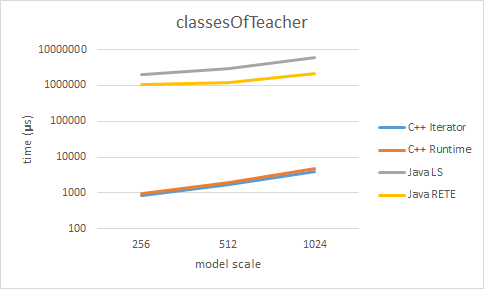
\includegraphics[width=120mm,
keepaspectratio]{figures/meas_classesOfTeacher.png}
\caption{Performance of the \emph{classesOfTeacher} query}
\label{fig:meas_classesOfTeacher}
\end{figure}

The next pattern is the \emph{studentsOfSchool}
(\listref{meas_studentOfSchool}), which is a moderately complex pattern. The
complexity comes from the fact that it is not possible to navigate through the
associations as described in the pattern because of the direction the
associations can be navigated in, thus the search plan has to overcome this via
starting from the center of the navigation chain and going in both directions
from there.

\begin{lstlisting}[frame=single,float=!ht,language=IQPL,
label=listing:meas_studentOfSchool, caption=The studentOfSchool pattern]
pattern studentsOfSchool(student, school) {
	Student.schoolClass.courses.school(student, school);
}
\end{lstlisting}

The more advanced pattern means the gap between the \CPP{} and Java
implementations became slightly smaller as seen on figure
\figref{meas_studentOfSchool}. As seen before, the Java local search
implementation still lags behind the RETE implementation.

\begin{figure}[!ht]
\centering
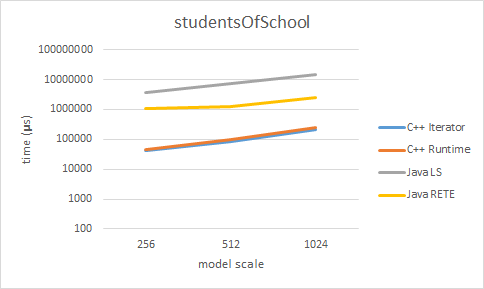
\includegraphics[width=120mm,
keepaspectratio]{figures/meas_studentOfSchool.png}
\caption{Performance of the \emph{studentOfSchool} query}
\label{fig:meas_studentOfSchool}
\end{figure}

The next pattern in line is the \emph{mutualFriendsInSchool}. This pattern is
the most complex of all the benchmarked patterns. The pattern searches for
two students in a single school whose friends with relationship is mutual. This
pattern is an absolute worst case scenario, as it calls an already complex
pattern twice resulting in a huge join at as the first steps of the search plan.

\begin{lstlisting}[frame=single,float=!ht,language=IQPL,
label=listing:meas_mutualFriendsInSchool, caption=The mutualFriendsInSchool pattern]
pattern mutualFriendsInOneSchool(studentA, studentB) {
	find studentsOfSchool(studentA, school);
	find studentsOfSchool(studentB, school);
	Student.friendsWith(studentA, studentB);
	Student.friendsWith(studentB, studentA);
}
\end{lstlisting}

In the case of this pattern the run times were a lot slower as expected,
which is why the times are written in milliseconds instead of microseconds
while the model scales are much smaller. The results, as seen on figure
\figref{meas_mutualFriendsInSchool}, do not continue the trend of the \CPP{}
version being faster than the Java implementation. In this case, both \CPP{}
implementations are slower then the Java RETE solution, while being slightly
faster than the Java local search version. The most likely reasons is a sub
optimal search plan, which more than likely significantly hurt the performance
of all local search based solutions.

\begin{figure}[!ht]
\centering
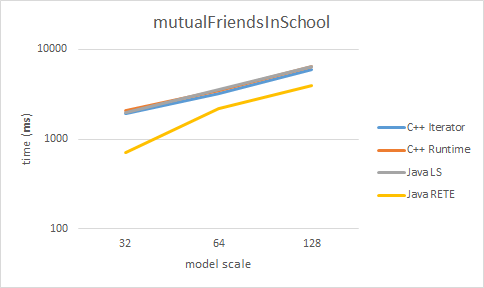
\includegraphics[width=120mm,
keepaspectratio]{figures/meas_mutualFriendsInSchool.png}
\caption{Performance of the \emph{mutualFriendsInSchool} query}
\label{fig:meas_mutualFriendsInSchool}
\end{figure}

The following figure (\figref{meas_second_run}) shows the times measured when
running the queries a second time. The pattern used in this benchmark is the
\emph{classesOfTeacher} (\listref{meas_classesOfTeacher}). In this case, the
\CPP{} implementations performed identical to the first run. The Java local
search based version shows slight massive improvements in its speed. The reason
for the speedup is that no preprocessing is necessary this time. The most
significant upgrade in speed is in the case of the Java RETE algorithm based
solution, as the times dropped to constant 1 ms independent from the model size.
This is because of the caching and incremental updating this algorithm is
capable of.

\begin{figure}[!ht]
\centering
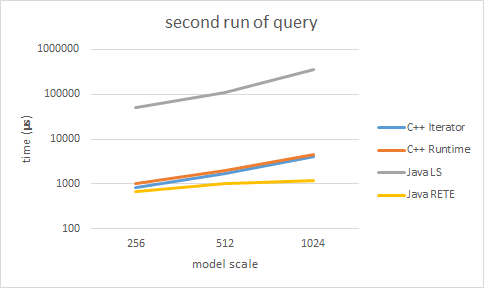
\includegraphics[width=120mm,
keepaspectratio]{figures/meas_second_run.png}
\caption{Performance of the second run of a query}
\label{fig:meas_second_run}
\end{figure}

The last figure (\figref{meas_runtime_vs_iterator}) demonstrates the
performance difference between the iterator based solution and the runtime based
one using the \emph{studentsOfSchool} pattern. The two solutions are qute close
to each other, they stay within 5-10\% of each other on most measurements with
the iterator based solution being the faster one. This is most likely because
it is not necessary to select the next search operation from an array as the
search operations are hard coded in the code.


\begin{figure}[!ht]
\centering
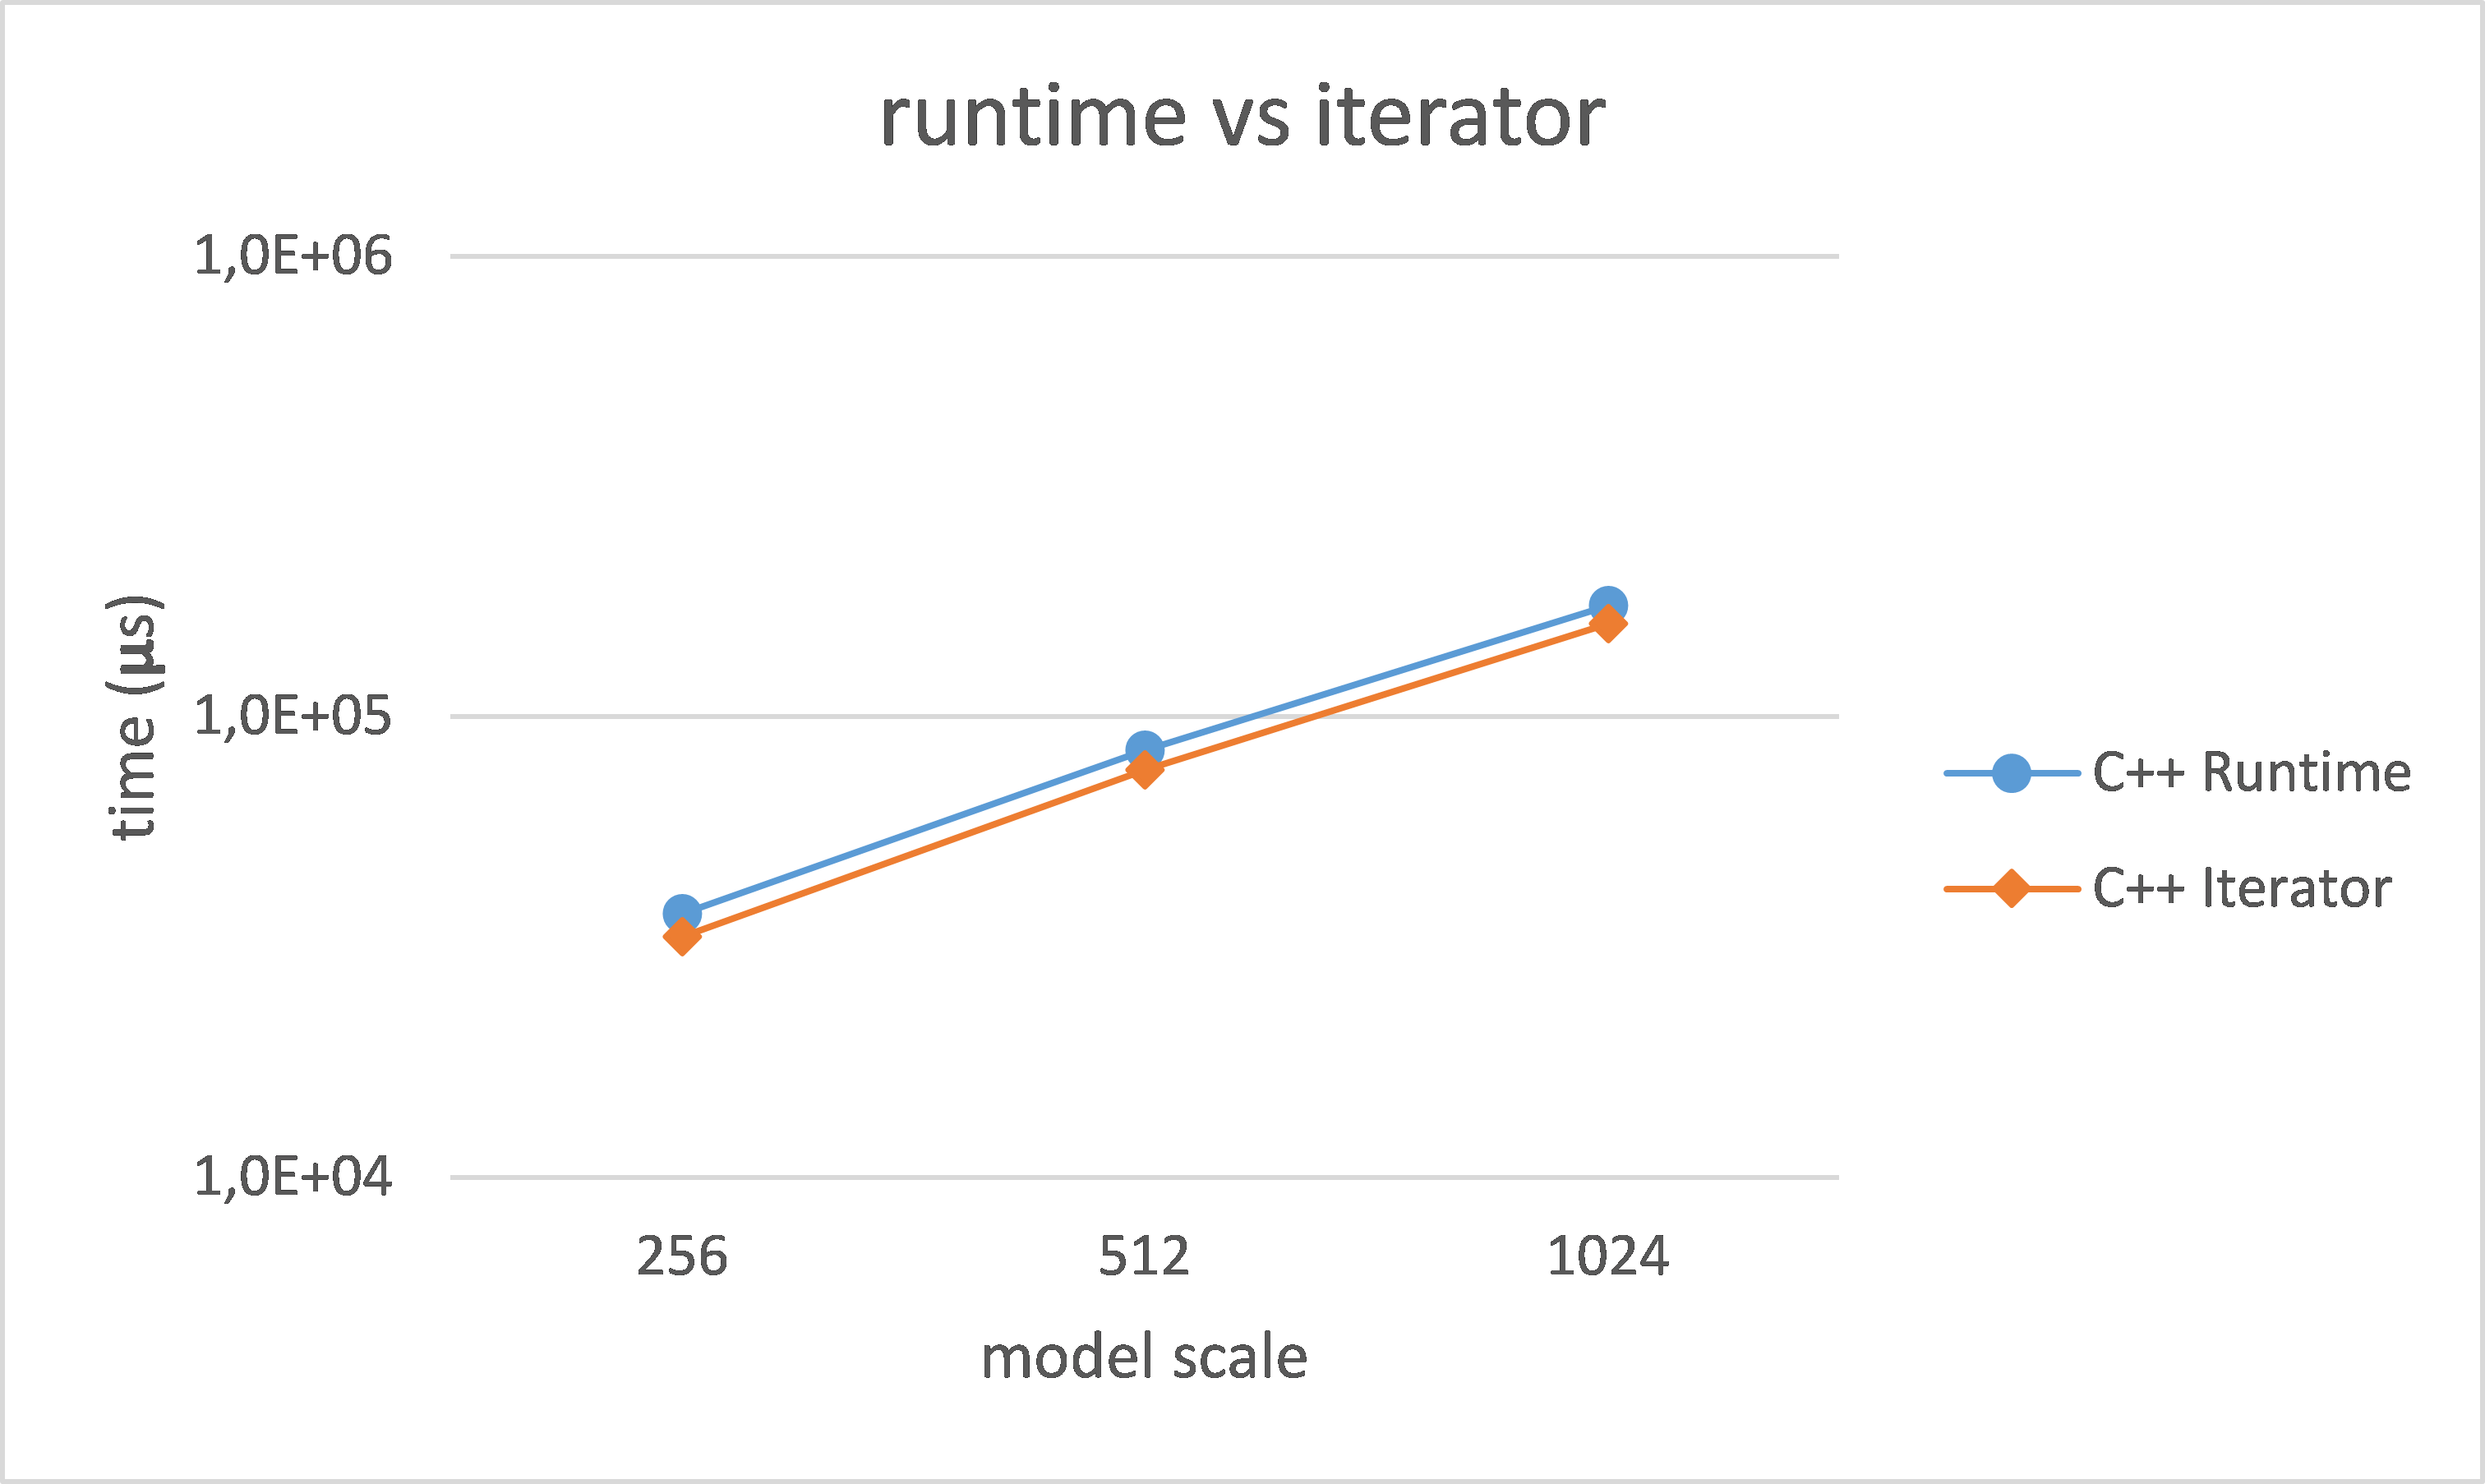
\includegraphics[width=120mm,
keepaspectratio]{figures/meas_runtime_vs_iterator.png}
\caption{Performance comparison of the runtime and iterator based implementations}
\label{fig:meas_runtime_vs_iterator}
\end{figure}

\chapter{Conclusion}

My job was to create an application capable of generating code from an EMF
model, able to declare queries over said model and run these queries over the
\CPP{} instances of the generated classes. I also had to test its scalability
and efficiency.

I managed to finish the following tasks:

\begin{itemize}
  \item Generating code from EMF model
  \item Generate search plan from the queries written in EMF-IncQuery Pattern
  Language
  \item Execution of the search plan over \CPP{} instances
  \item Scaleability and performance testing
\end{itemize}

During my work I did not manage to implement every feature of the original
\EIQ{} engine, as the handling of constants, evaluation and check
expressions and negative pattern application is still missing. The negative
pattern applications could be implemented by generating a version of the
negatively applied pattern where all the parameters are bound, calling this and
checking if there are any matches as a search operation. The check and eval
operations are more problematic, as they would require the modification of the
pattern language. The \EIQ{} pattern language allows the writing of check
expression using the Xbase language, which allows the usage of Java libraries.
Translating this to Java would be unreasonable amount of work, thus restricting
the usable expression is the better solution.

Throughout development, the fact that the Java local search engine was
still being implemented slowed down my job a significantly. There were several
occasions when a bug in the search plan generation would break the \CPP{}
generated code, components did not behave as documented or the Java API was not
planned with external contributions in mind, resulting in temporary hacks and
workarounds.

There are still a lot of work left to be done on the resulting program. The
generated code should is currently not tested, this resulted in many unexpected
bugs when encountering with specific edge cases. Another possible improvement
would be the implementation of a multithreaded version of the search plan
execution. This could result in significant performance gains in the case of
larger models and more complex queries. In addition, it would be worthwhile to
check different ways of solving the \CPP{} related problems mentioned in section
\sectref{CppSpecificProblems}. For example it might be a reasonable restraint
for all of the model classes to inherit from a common base type, as \CPP{}
allows for multiple inheritance.

All in all, I believe the resulting program, while definitely not production
ready, proved that it might be worthwhile to put further research and
development in the \CPP{} implementation of search plan execution, as the
measured performance was significantly better in most cases.


\bibliography{mybib}
\addcontentsline{toc}{chapter}{Bibliography}
\bibliographystyle{plain}

%%----------------------------------------------------------------------------
\appendix
%----------------------------------------------------------------------------
\chapter*{Appendix}\addcontentsline{toc}{chapter}{Appendix}

\label{page:last}
\end{document}
